\documentclass{article}
\usepackage{graphicx}
\usepackage{wrapfig}
\usepackage{amsmath}
\usepackage{verbatim}
\usepackage{makeidx}

\title{Programming the iMobot}  
%\author{David Ko\\Mechanical and Aerospace Engineering}
%\date{\today} 
\makeindex

\begin{document}
\maketitle

\section{The \texttt{CMobot} iMobot Remote Control Library}
The \texttt{CMobot} library is a collection of functions geared towards
controlling the motors and reading sensor values of an iMobot module via the
Bluetooth wireless protocol. The functions are designed to be intuitive
and easy to use. Various functions are provided to control or obtain the speed,
direction, and position of the motors. The API includes C-style functions as well
as a C++ class called \texttt{CMobot} to facilitate C++ style api function
calls. 

This documentation introduces the basic computer setup required for controlling 
the iMobot, as well as several demo programs and a complete reference for all
API function provided with the \texttt{CMobot} library.

\section{\label{sec:pairing}Bluetooth Pairing with the iMobot}
To control the iMobot with the Bluetooth wireless protocol, the controlling 
computer must be equipped with Bluetooth. If the computer does not have
Bluetooth built-in, an external USB Bluetooth dongle may be used. The following
instructions are for a Windows 7 computer with built-in Bluetooth. The basic
process is the same for Windows XP and Vista, although the screenshots may
appear different. 

The first step is to open the Bluetooth applet by double-clicking the Bluetooth
icon in the applet tray normally found at the bottom right of the screen, as
shown highlighted in red in the following figure.

\begin{center}

\includegraphics[width=3in]{images/imobot_connect_1.png}
\end{center}

After double-clicking the icon, a new window will appear similar to the following.

\begin{center}
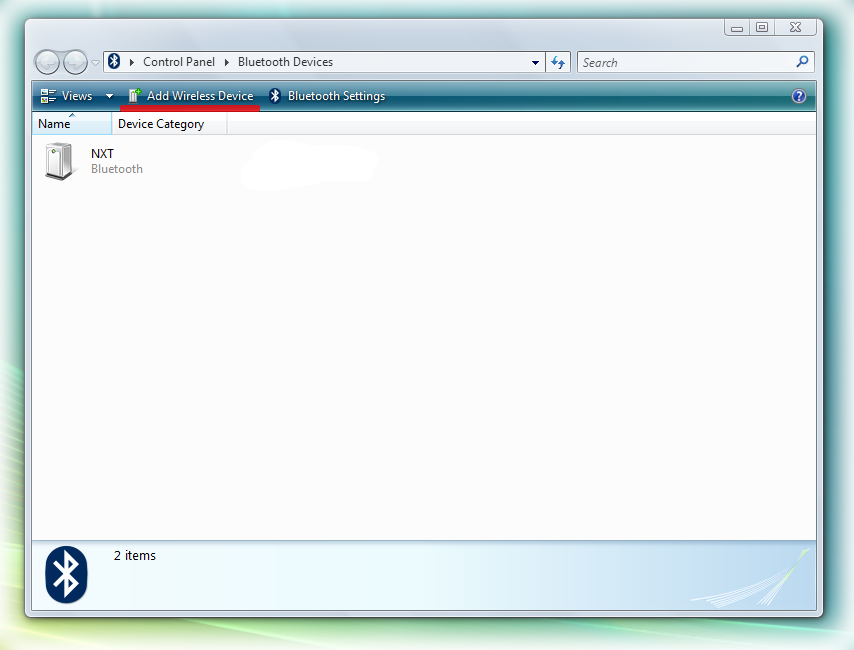
\includegraphics[width=5in]{images/imobot_connect_1a.png}
\end{center}

Next, click on the
button labeled "Add Wireless Device" towards the top of the window. This 
will bring up the following dialog.

\begin{center}
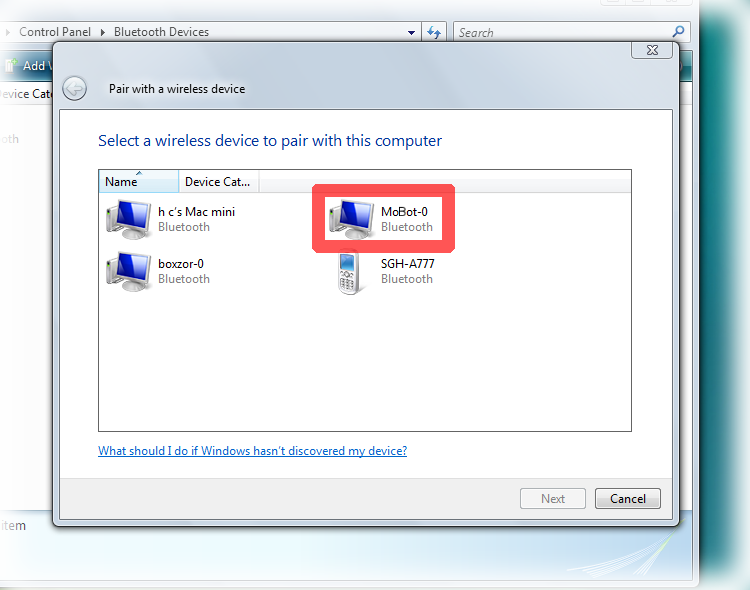
\includegraphics[width=5in]{images/imobot_connect_2.png}
\end{center}

This dialog shows a list of all Bluetooth wireless devices that are in range.
Among them should be the iMobot you wish to connect to. If the iMobot does not
appear on this list, please ensure that the iMobot is within 10 meters of the
connecting computer and that the iMobot is powered on. Double click on the icon
representing the iMobot to proceed. Once you have double-clicked the icon, the
following dialog box should appear.

\begin{center}
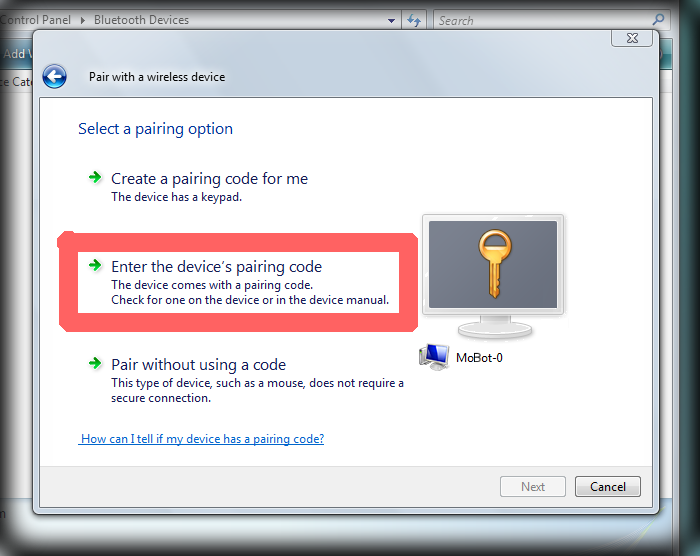
\includegraphics[width=5in]{images/imobot_connect_3.png}
\end{center}

Select the second option, labeled ``Enter the device's pairing code''. iMobot
modules come hard-coded with a default pairing code. When prompted for the
pairing code, enter ``1234''. Once the computer is paired with the iMobot,
the following dialog box may pop up asking to install drivers.

\begin{center}
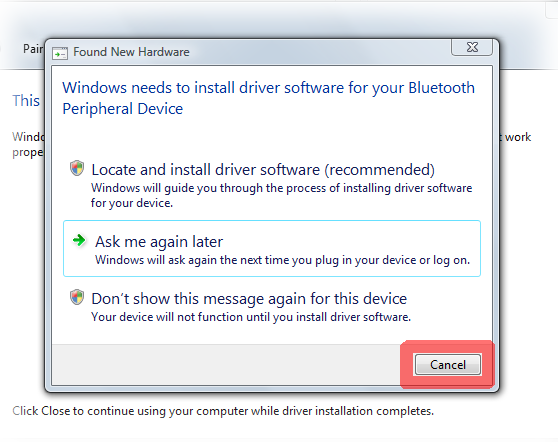
\includegraphics[width=5in]{images/imobot_connect_4.png}
\end{center}

If the previously illustrated dialog box appears, just click the ``cancel''
button at the bottom right. No extra drivers are necessary for controlling the
iMobot module.

At this point, the following dialog should be shown.

\begin{center}
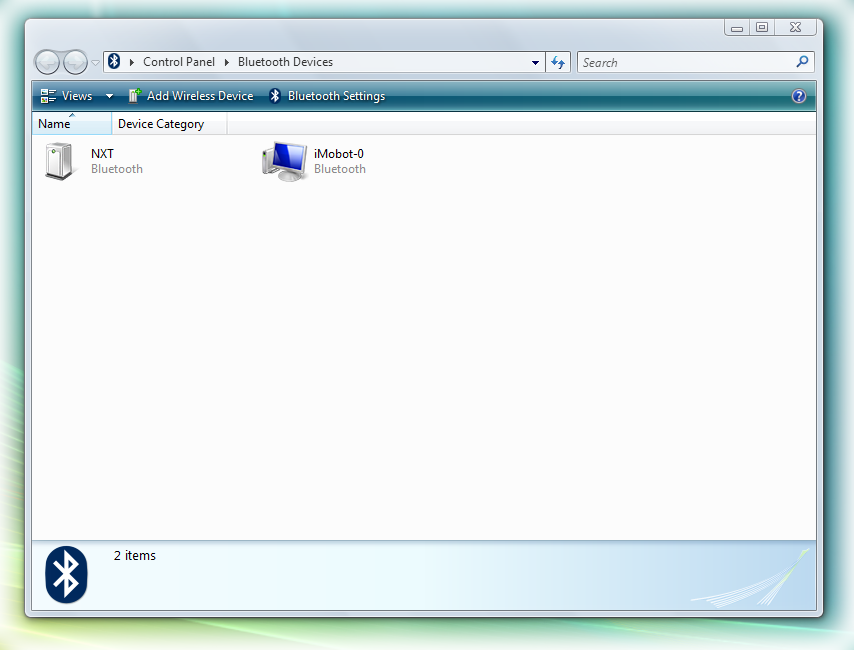
\includegraphics[width=5in]{images/imobot_connect_6.png}
\end{center}

The next step is to enable the iMobot control service. 
Double-click on the icon denoting the
iMobot module to bring up the following dialog:

\begin{center}
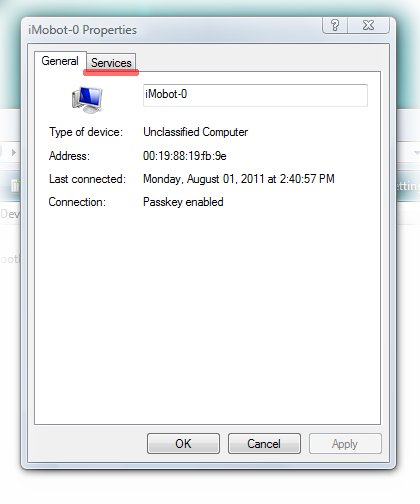
\includegraphics[width=5in]{images/imobot_connect_7.png}
\end{center}

Click on the tab labeled ``Services''

\begin{center}
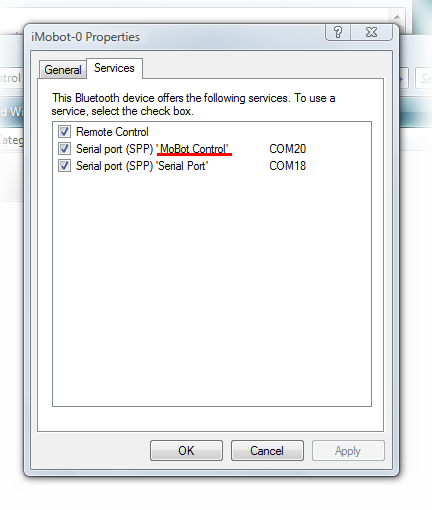
\includegraphics[width=5in]{images/imobot_connect_8.png}
\end{center}

Ensure that the service titled ``iMobot Control'' is enabled. If it is not
enabled, click on the check-box to enable it. Click on the ``Ok'' button to
accept the changes and close the dialogs. The iMobot is now ready to be
controlled with the iMobotComms library.

\section{ The MoBot Remote Control Program }
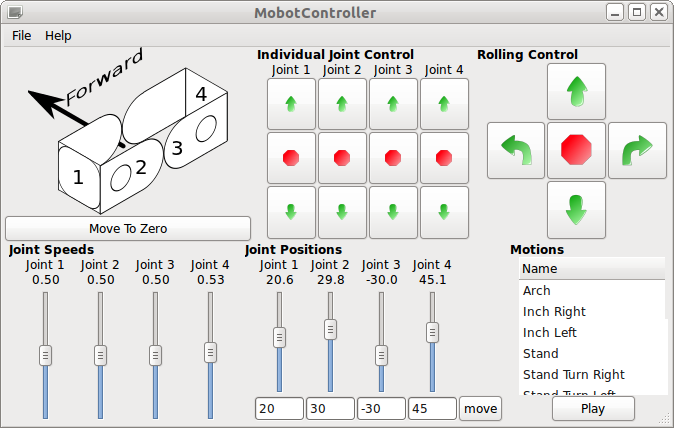
\includegraphics[width=4.5in]{images/iMobot_controller_screenshot.png}

The preceding figure shows the MoBot remote control program. The
program displays a graphical interface which may be used to display
information about the iMobot's joint positions, and also control the
speeds and positions of the MoBot's joints. The interface is divided
up into six sections; three on the top half of the interface, and three on 
the bottom half. 

\subsection{The iMobot Diagram and ``Move To Zero'' Button}
The first section of the GUI located on the top left of the interface
displays a schematic diagram of the iMobot, displaying motor positions.
Underneath the diagram, there is a large button with the text 
``Move To Zero''. When clicked, this button will command the connected
MoBot to rotate all of its joints to a flat ``Zero'' position.

\subsection{Individual Joint Control}
The second section, located at the top-middle section of the interface,
is the ``Individual Joint Control'' section. These buttons command the
MoBot to move individual joints. When the up or down arrows are clicked,
the MoBot begins to move the corresponding joint in either the positive,
or negative direction. The joint will continue to move until the stop 
button, located between the up and down arrows, is clicked. 

\subsection{Rolling Control}
This section contains buttons for controlling the iMobot as a 
two wheeled mobile robot. The up and down buttons cause the MoBot to
roll forward or backward. The left and right buttons cause the MoBot 
to rotate towards the left, or towards the right. The stop button in the
middle causes the MoBot to stop where it is.

\subsection{Joint Speeds}
The ``Joint Speeds'' section, located at the bottom left of the interface,
displays and controls the current joint speeds of the MoBot. Joint speeds
are a value between 0 and 1, with 1 meaning maximum joint power, and 0
meaning zero joint power. The speed may be set by sliding the vertical 
sliders to the desired positions. 

\subsection{Joint Positions}
This section, located in the bottom-middle of the interface, is used to display
and control the positions of each of the four
joints of a MoBot. The joint positions are displayed in the numerical
text located above each vertical slider. The displayed joint positions are in
units of degrees.  There are two methods to control
the joints using this interface.

The first method of controlling the joints is by using the vertical sliders.
Each vertical slider's position represents a joint's angle. The sliders for the
two end joints vary from -180 degrees to 180 degrees, representing one complete
rotation. The angles for the two body joints vary from -90 to 90 degrees. When
the position of the slider is moved, the MoBot will move its joints to match the 
sliders. 

The second method for moving the joints is by entering the exact angles for the
joints. Below each of the four sliders lies a text entry box. Values in degrees
may be typed into each of the four entry boxes. When the button on the lower
right of the section labeled ``Move'' is clicked, the MoBot will move its joints
to match the values typed into the boxes. If no value is typed into a box, that 
joint will not move.

\subsection{Motions}
This section, located on the bottom right of the interface, contains a set of
preprogrammed motions for the MoBot. To execute a preprogrammed motion, simply
click on the name of the motion you wish to execute, and then click the button
labeled ``Play''.

\section{Basics of a Ch iMobot Program}
To help the user become acquainted with the iMobot control programs, one sample
program will be presented to illustrate the basics and minimum requirements of
an iMobot control program. 

\subsection{\texttt{getting\_started.ch} Source Code}
\verbatiminput{../demos/getting_started/getting_started.ch}

\subsection{\label{sec:democode}Demo Code for \texttt{getting\_started.ch} Explained}
The beginning of every iMobot control program will include header files. Each
header file imports functions used for a number of tasks, such as printing
data onto the screen or controlling the iMobot. 

\begin{verbatim}
#include <mobot.h> // Required for iMobot control functions
\end{verbatim}

Next, we must initialize the C++ class used to control the iMobot. This line
initializes a new variable named \texttt{robot} which represents the remote
iMobot module which we wish to control. This special variable is actually an
instance of the \texttt{CMobot} class, which contains its own set of
functions called ``methods'' or ``member functions''.
\begin{verbatim}
CMobot robot;
\end{verbatim}
Note that there is an alternative way to create the \texttt{robot} variable.
The alternate method takes the following syntax:
\begin{verbatim}
CMobot robot("12:34:56:78:90:12", 20);
\end{verbatim}
The alternate syntax instructs the new \texttt{CMobot} variable named 
\texttt{robot} to explicitely connect to the robot with address
\texttt{"12:34:56:78:90:12"} and channel \texttt{20}. This method allows
the iMobot program to connect to an iMobot even if it has not been paired,
as described in Section \ref{sec:pairing}. However, it requires the user
to know the Bluetooth address of the iMobot in advance.

The next line will use the \texttt{moveToZero} member function. The
\texttt{moveToZero} function causes the iMobot to move all of its motors to the
zero position.
\begin{verbatim}
robot.moveToZero();
\end{verbatim}

The majority of iMobot control functions do not wait for the robotic motions to
complete before continuing. As such, if we want to wait for the robot to fully
complete the requested motion before continuing with the rest of the program,
we must use the \texttt{moveWait} function, as such.
\begin{verbatim}
robot.moveWait();
\end{verbatim}

The next four lines of code command joints 1 and 4 to rotate 90 degrees, and
then waits for the motors to stop moving. Joints 1 and 4 are the faceplates
of the iMobot which are sometimes used to act as "wheels".
\begin{verbatim}
robot.moveJointTo(IMOBOT_JOINT1, 90);
robot.moveJointTo(IMOBOT_JOINT4, 90);
robot.moveJointWait(IMOBOT_JOINT1);
robot.moveJointWait(IMOBOT_JOINT4);
\end{verbatim}

\section{Preprogrammed Motions}
The MoBot API contains functions for executing preprogrammed motions. The 
preprogrammed motions are motions which are commonly used for MoBot locomotion.
Following is a list of available functions and a brief description about
their effect on the MoBot.
\begin{itemize}
\item \texttt{motionInchwormLeft()}: This function causes the MoBot to perform
  the inchworm gait once, moving the MoBot towards its left.
\item \texttt{motionInchwormRight()}: This function causes the MoBot to perform
  the inchworm gait once, moving the MoBot towards its right.
\item \texttt{motionRollBackward()}: This function causes the MoBot to rotate
  its faceplates, using them as wheels to roll backward.
\item \texttt{motionRollForward()}: This function causes the MoBot to rotate
  its faceplates, using them as wheels to roll forward.
\item \texttt{motionStand()}: This function causes the MoBot to stand up onto a 
  faceplate, assuming the camera platform position.
\item \texttt{motionTurnLeft()}: Uses the MoBot's faceplates as wheels, turning
  them in opposite directions in order to rotate the MoBot towards its left.
\item \texttt{motionTurnRight()}: Uses the MoBot's faceplates as wheels, turning
  them in opposite directions in order to rotate the MoBot towards its right.
\end{itemize}

\section{Blocking and Non-Blocking Functions}
All of the MoBot movement functions may be designated as either ``blocking'' 
functions or ``nonblocking'' functions. A blocking function is a function which
does not return while operations are being performed. For instance, the
\texttt{moveWait()} function is a blocking function. When called, the function
will hang, or ``block'', until all the joints have stopped moving.

The function \texttt{move()} is an example of a non-blocking function. When
the \texttt{move()} function is called, the function immediately returns 
as the joints begin moving. The next statement in the program is executed
even before the movement has completed. 

\subsection{List of Non-Blocking Movement Functions}
\begin{itemize}
\item \texttt{move()}
\item \texttt{moveContinuous()}
\item \texttt{moveJointTo()}
\item \texttt{moveTo()}
\item \texttt{moveToZero()}
\end{itemize}

\subsection{List of Blocking Movement Functions}
\begin{itemize}
\item \texttt{moveContinuousTime()}
\item \texttt{moveJointWait()}
\item \texttt{moveWait()}
\item \texttt{motionInchwormLeft()}
\item \texttt{motionInchwormRight()}
\item \texttt{motionRollBackward()}
\item \texttt{motionRollForward()}
\item \texttt{motionStand()}
\item \texttt{motionTurnLeft()}
\item \texttt{motionTurnRight()}
\end{itemize}

\newpage
\appendix
\section{iMobotComms API}
%\lhead{libimobotcomms API Documentation}
\noindent
The header file {\bf mobot.h} defines all the data types, macros 
and function prototypes for the mobot API library. The header file
declares a class called \texttt{CMobot} which contains member functions which
may be used to control the mobot.

\begin{table}[!h]
%\capstart
\begin{center}
\caption{CMobot Member Functions.}
\begin{tabular}{p{48 mm}p{110 mm}}
%\begin{tabular}{ll}
\hline
Function & Description \\
\hline
%\texttt{pose()} \dotfill & Pose multiple joints of the mobot. \\
\texttt{CMobot()} & The CMobot constructor function. This function
is called automatically and should not be called explicitly. \\
\texttt{\textasciitilde CMobot()} & The CMobot destructor function. This function
is called automatically and should not be called explicitly. \\
& \\
\texttt{blinkLED()} & Blink the LED on a Mobot module. \\
\texttt{connect()} & Connect to a remote mobot module. This function 
connects to the first mobot listed in the Barobo configuration file. To
edit the configuration file, use the mobot control graphical user interface,
and select the menu item ``Mobot $\rightarrow$ Configure Mobot Bluetooth''. \\
\texttt{connectWithBluetoothAddress()} & Connect to a mobot module by specifying its Bluetooth address. \\
\texttt{connectWithIPAddress()} & Connect to a mobot module by specifying a remote computer's IP address. \\
\texttt{disconnect()} & Disconnect from a mobot module. \\
\texttt{disableButtonCallback()} & Reverts a Mobot's buttons to their factory-default functions. \\
\texttt{driveTo()} & Move all four joints of the mobot to specified absolute angles. \\
\texttt{driveToNB()} & Move all four joints of the mobot to specified absolute angles. \\
\texttt{enableButtonCallback()} & Enables a user-driven callback for handling button-press events on a module. \\
\texttt{getJointAngle()} & Get a joint's angle. \\
\texttt{getJointAngles()} & Get joint angles for all joints. \\
%\texttt{getJointDirection()} & Gets a motor's currently assigned direction. \\
\texttt{getJointMaxSpeed()} & Get a joint's maximum speed in radians per second. \\
\texttt{getJointSafetyAngle()} & Get the mobot's safety angle limit. \\
\texttt{getJointSafetyAngleTimeout()} & Get the mobot's safety angle limit timeout. \\
\texttt{getJointSpeed()} & Get a motor's current speed setting in radians per second. \\
\texttt{getJointSpeeds()} & Get all motor's current speed settings in radians per second. \\
\texttt{getJointSpeedRatio()} & Get a motor's speed as a ratio of the motor's maximum speed. \\
\texttt{getJointSpeedRatios()} & Get all motor speeds as ratios of the motor's maximum speed. \\
\texttt{getJointState()} & Get a motor's current status. \\
\texttt{isConnected()} & This function is used to check the connection to a mobot. \\
\texttt{isMoving()} & This function is used to check if any joints are currently in motion. \\
\texttt{move()} & Move all four joints of the mobot by specified angles. \\
\texttt{moveNB()} & Identical to \texttt{move()} but non-blocking. \\
\texttt{moveContinuousNB()} & Move joints continuously. Joints will move untill stopped.\\
\texttt{moveContinuousTime()} & Move joints continuously for a certain amount of time.\\
\texttt{moveJoint()} & Move a joint. \\
\texttt{moveJointContinuousNB()} & Move a joint continuously. \\
\texttt{moveJointContinuousTime()} & Move a joint continuously for a certain amount of time. \\
\texttt{moveJointNB()} & Move a joint. \\
\texttt{moveJointTo()} & Set the desired motor position for a joint. \\
\texttt{moveJointToNB()} & Identical to \texttt{moveJointTo()} but non-blocking. \\
\texttt{moveJointWait()} & Wait until the specified motor has stopped moving. \\
\texttt{moveTo()} & Move all four joints of the mobot to specified absolute angles. \\
\texttt{moveToNB()} & Identical to \texttt{moveTo()} but non-blocking. \\
\texttt{moveToZero()} & Instruct all motors to go to their zero positions. \\
\texttt{moveToZeroNB()} & Identical to \texttt{moveToZero()} but non-blocking. \\
\texttt{moveWait()} & Wait until all motors have stopped moving. \\
%\texttt{setJointDirection()} & Set the motor direction of a motor. Set
%to "0" for automatic direction, "1" for forward, and "2" for reverse. \\
\texttt{recordAngle()} & Begin recording the angle of a joint. \\
\texttt{recordAngleBegin()} & Begin recording the angle of a joint. \\
\texttt{recordAngleEnd()} & End recording the angle of a joint. \\
\texttt{recordAngles()} & Begin recording the angle of all joints. \\
\texttt{recordAnglesBegin()} & Begin recording the angle of all joints. \\
\texttt{recordAnglesEnd()} & End recording the angle of all joints. \\
\texttt{recordWait()} & Wait for recording operations to finish. \\
\hline
\end{tabular}
\end{center}
\label{mobilec_api_cbinary}
\end{table}

\addtocounter{table}{-1}

\begin{table}[!h]
%\capstart
\begin{center}
\caption{CMobot Member Functions (Continued)}
\begin{tabular}{p{48 mm}p{110 mm}}
%\begin{tabular}{ll}
\hline
Function & Description \\
\hline
\texttt{resetToZero()} & Instruct all motors to go to their zero positions. \\
\texttt{setJointMovementStateNB()} & Set the movement state of a joint. \\
\texttt{setJointMovementStateTime()} & Set the movement state of a joint for a period of time.\\
\texttt{setJointSafetyAngle()} & Set the mobot's safety angle limit. The default value is 10 degrees.\\
\texttt{setJointSafetyAngleTimeout()} & Set the mobot's safety angle limit timeout. The default value is 0.5 seconds.\\
\texttt{setJointSpeed()} & Set a motor's speed setting in radians per second. \\
\texttt{setJointSpeeds()} & Set all motor speeds in radians per second. \\
\texttt{setJointSpeedRatio()} & Set a joints speed setting to a fraction of its maximum speed, a value between 0 and 1. \\
\texttt{setJointSpeedRatios()} & Set all joint speed settings to a fraction of its
maximum speed, expressed as a value from 0 to 1. \\
\texttt{setMovementStateNB()} & Change the movement states of the joints. Movement states include moving forward, backward, neutral, or holding their current position.\\
\texttt{setMovementStateTime()} & Change the movement states of the joints for a certain amount of time.\\
\texttt{stopAllJoints()} & Stop all currently executing motions of the mobot. \\
\texttt{stopOneJoint()} & Stop a joint on the mobot. \\
\texttt{stopTwoJoints()} & Stop two joints on the mobot. \\
\texttt{stopThreeJoints()} & Stop three joints on the mobot. \\
\hline
\end{tabular}
\end{center}
\label{mobilec_api_cbinary}
\end{table}

\begin{table}[!h]
%\capstart
\begin{center}
\caption{CMobot Member Functions for Compound Motions.}
\begin{tabular}{p{38 mm}p{107 mm}}
Compound Motions & These are convenience functions of commonly used compound motions. \\
\hline
\texttt{motionArch()} \dotfill & Arch the mobot for better ground clearance. \\
\texttt{motionArchNB()} \dotfill & Identical to \texttt{motionArch} but non-blocking. \\
\texttt{motionInchwormLeft()} \dotfill & Inchworm motion towards the left. \\
\texttt{motionInchwormLeftNB()} \dotfill & Identical to \texttt{motionInchwormLeft} but non-blocking. \\
\texttt{motionInchwormRight()} \dotfill & Inchworm motion towards the right. \\
\texttt{motionInchwormRightNB()} \dotfill & Identical to \texttt{motionInchwormRight} but non-blocking. \\
\texttt{motionRollBackward()} \dotfill & Roll on the faceplates toward the backward direction. \\
\texttt{motionRollBackwardNB()} \dotfill & Identical to \texttt{motionRollBackward()} but non-blocking. \\
\texttt{motionRollForward()} \dotfill & Roll on the faceplates forwards. \\
\texttt{motionRollForwardNB()} \dotfill & Identical to \texttt{motionRollForward()} but non-blocking. \\
\texttt{motionSkinny()} \dotfill & Move the mobot into a skinny profile. \\
\texttt{motionSkinnyNB()} \dotfill & Identical to \texttt{motionSkinny()} but non-blocking. \\
\texttt{motionStand()} \dotfill & Stand the mobot up on its end. \\
\texttt{motionStandNB()} \dotfill & Identical to \texttt{motionStand()} but non-blocking. \\
\texttt{motionTumbleLeft()} \dotfill & Perform the tumbling motion. \\
\texttt{motionTumbleLeftNB()} \dotfill & Identical to \texttt{motionTumbleLeft()} but non-blocking. \\
\texttt{motionTumbleRight()} \dotfill & Perform the tumbling motion in the opposite direction of ``motionTumbleLeft''. \\
\texttt{motionTumbleRightNB()} \dotfill & Identical to \texttt{motionTumbleRight()} but non-blocking. \\
\texttt{motionTurnLeft()} \dotfill & Rotate the mobot counterclockwise. \\
\texttt{motionTurnLeftNB()} \dotfill & Identical to \texttt{motionTurnLeft()} but non-blocking. \\
\texttt{motionTurnRight()} \dotfill & Rotate the mobot clockwise. \\
\texttt{motionTurnRightNB()} \dotfill & Identical to \texttt{motionTurnRight()} but non-blocking. \\
\texttt{motionWait()} \dotfill & Wait for a motion to finish. \\
\hline
\end{tabular}
\end{center}
\label{mobilec_api_compound}
\end{table}

\clearpage
\newpage
\noindent
\vspace{5pt}
\rule{4.5in}{0.015in}\\
\noindent
{\LARGE \texttt{CMobot::blinkLED()}\index{CMobot::blinkLED()}}\\
%\phantomsection
\addcontentsline{toc}{section}{blinkLED()}

\noindent
{\bf Synopsis}
\vspace{-8pt}
\begin{verbatim}
#include <mobot.h>
int CMobot::blinkLED(double delay, int numBlinks);
\end{verbatim}

\noindent
{\bf Purpose}\\
Blink the on-board LED on a Mobot module.\\

\noindent
{\bf Return Value}\\
The function returns 0 on success and non-zero otherwise.\\

\noindent
{\bf Parameters}\\
\vspace{-0.1in}
\begin{description}
\item               
\begin{tabular}{p{15 mm}p{125 mm}}
\texttt{delay} & The amount of time between blinks. \\
\texttt{numBlinks} & The number of times to blink the LED. \\
\end{tabular}
\end{description}
\noindent
{\bf Description}\\
This function is used to blink or flash the LED on a Mobot module. The first
argument, \texttt{delay}, is used to control the speed of the blinking
LED, and the second argument, \texttt{numBlinks}, controls the number of times
to blink. For instance, the line
\begin{verbatim}
mobot.blinkLED(0.1, 10);
\end{verbatim}
would cause a mobot to blink 10 times fast, and the line
\begin{verbatim}
mobot.blinkLED(1, 2);
\end{verbatim}
would cause the mobot to do two slow blinks.

\noindent
{\bf Example}\\
\noindent

\noindent
{\bf See Also}\\

%\CPlot::\DataThreeD(), \CPlot::\DataFile(), \CPlot::\Plotting(), \plotxy().\\

\noindent
\vspace{5pt}
\rule{4.5in}{0.015in}\\
\noindent
{\LARGE \texttt{CMobot::connect()}\index{connect()}}\\
%\phantomsection
\addcontentsline{toc}{section}{connect()}

\noindent
{\bf Synopsis}\\
\begin{verbatim}
#include <mobot.h>
int CMobot::connect();
\end{verbatim}

\noindent
{\bf Purpose}\\
Connect to a remote iMobot via Bluetooth.\\

\noindent
{\bf Return Value}\\
The function returns 0 on success and non-zero otherwise.\\

\noindent
{\bf Parameters}\\
None.\\

\noindent
{\bf Description}\\
This function is used to connect to an iMobot. The iMobot must first be paired
with the computer. This function currently only works in Microsoft Windows
operating systems. For other operating systems, please use the
\texttt{connectAddress()} function.

\noindent
{\bf Example}\\
Please see the example in Section \ref{sec:democode} on page \pageref{sec:democode}.\\
\noindent

\noindent
{\bf See Also}\\
\texttt{connectAddress()}

%\CPlot::\DataThreeD(), \CPlot::\DataFile(), \CPlot::\Plotting(), \plotxy().\\

\noindent
\vspace{5pt}
\rule{4.5in}{0.015in} \\
\noindent
{\LARGE \texttt{CMobot::connectWithBluetoothAddress()}\index{CMobot::connectWithBluetoothAddress()}}\\
%\phantomsection
\addcontentsline{toc}{section}{connectWithBluetoothAddress()}

\noindent
{\bf Synopsis}
\vspace{-8pt}
\begin{verbatim}
#include <mobot.h>
int CMobot::connectWithBluetoothAddress(char address[], int channel = 1);
\end{verbatim}

\noindent
{\bf Purpose}\\
Connect to a remote mobot via Bluetooth by specifying the specific Bluetooth
address of the device.\\

\noindent
{\bf Return Value}\\
The function returns 0 on success and non-zero otherwise.\\

\noindent
{\bf Parameters}
\vspace{-0.1in}
\begin{description}
\item               
\begin{tabular}{p{10 mm}p{145 mm}}
\texttt{address} & The Bluetooth address of the mobot. \\
\texttt{channel} & (optional) The Bluetooth channel that the listening program is
listening on. The default channel is channel 1. \\
\end{tabular}
\end{description}

\noindent
{\bf Description}\\
This function is used to connect to a mobot. 

\noindent
{\bf Example}\\
\begin{verbatim}
mobot.connectWithBluetoothAddress("00:06:66:45:DA:02", 1);
mobot.connectWithBluetoothAddress("00:06:66:45:DA:F3");
\end{verbatim}
\noindent

\noindent
{\bf See Also}\\
\texttt{connect(), disconnect()}

%\CPlot::\DataThreeD(), \CPlot::\DataFile(), \CPlot::\Plotting(), \plotxy().\\

\noindent
\vspace{5pt}
\rule{4.5in}{0.015in} \\
\noindent
{\LARGE \texttt{CMobot::connectWithIPAddress()}\index{CMobot::connectWithIPAddress()}}\\
%\phantomsection
\addcontentsline{toc}{section}{connectWithIPAddress()}

\noindent
{\bf Synopsis}
\vspace{-8pt}
\begin{verbatim}
#include <mobot.h>
int CMobot::connectWithIPAddress(char address[], char port[] = "5768");
\end{verbatim}

\noindent
{\bf Purpose}\\
Connect to a remote mobot connected to a remote computer over the internet.\\

\noindent
{\bf Return Value}\\
The function returns 0 on success and non-zero otherwise.\\

\noindent
{\bf Parameters}
\vspace{-0.1in}
\begin{description}
\item               
\begin{tabular}{p{10 mm}p{145 mm}}
\texttt{address} & The IP address of the remote computer. \\
\texttt{port} & (optional) The port to connect to. \\
\end{tabular}
\end{description}

\noindent
{\bf Description}\\
This function is used to connect to a mobot. 

\noindent
{\bf Example}\\
mobot.connectWithIPAddress("192.168.0.132", "8734");
mobot.connectWithIPAddress("mobots.example.com", "5768");
mobot.connectWithIPAddress("192.168.100.221");
\noindent

\noindent
{\bf See Also}\\
\texttt{connect(), disconnect()}

%\CPlot::\DataThreeD(), \CPlot::\DataFile(), \CPlot::\Plotting(), \plotxy().\\

\noindent
\vspace{5pt}
\rule{4.5in}{0.015in}\\
\noindent
{\LARGE \texttt{CMobot::disconnect()}\index{CMobot::disconnect()}}\\
%\phantomsection
\addcontentsline{toc}{section}{disconnect()}

\noindent
{\bf Synopsis}\\
\begin{verbatim}
#include <mobot.h>
int CMobot::disconnect();
\end{verbatim}

\noindent
{\bf Purpose}\\
Disconnect from a remote robot.\\

\noindent
{\bf Return Value}\\
The function returns 0 on success and non-zero otherwise.\\

\noindent
{\bf Parameters}\\
None.\\

\noindent
{\bf Description}\\
This function is used from disconnect to a robot. A call to this function is
not necessary before the termination of a program. It is only necessary if
another connection will be established within the same program at a later time.
\\

\noindent
{\bf Example}\\
\noindent

\noindent
{\bf See Also}\\
\texttt{connect(), connectWithAddress()}

%\CPlot::\DataThreeD(), \CPlot::\DataFile(), \CPlot::\Plotting(), \plotxy().\\

\noindent
\vspace{5pt}
\rule{4.5in}{0.015in}\\
\noindent
{\LARGE \texttt{CMobot::driveJointTo()}\index{CMobot::driveJointTo()}}\\
{\LARGE \texttt{CMobot::driveJointToNB()}\index{CMobot::driveJointToNB()}}\\
%\phantomsection
\addcontentsline{toc}{section}{driveJointTo()}
\addcontentsline{toc}{section}{driveJointToNB()}

\noindent
{\bf Synopsis}
\vspace{-8pt}
\begin{verbatim}
#include <mobot.h>
int CMobot::driveJointTo(moboJointId_t id, double angle);
int CMobot::driveJointToNB(moboJointId_t id, double angle);
\end{verbatim}

\noindent
{\bf Purpose}\\
Move all of the joints of a mobot to the specified positions.\\

\noindent
{\bf Return Value}\\
The function returns 0 on success and non-zero otherwise.\\

\noindent
{\bf Parameters}\\
\vspace{-0.1in}
\begin{description}
\item               
\begin{tabular}{p{15 mm}p{105 mm}}
\texttt{id} & The id of the joint to move. \\
\texttt{angle} & The absolute position to move the joint, expressed in degrees. \\
\end{tabular}
\end{description}
\noindent

{\bf Description}\\
\vspace{-12pt}
\begin{quote}
Note that this function is similar to the \texttt{moveJointTo()} family of functions, except
that this variant ignores the speed settings of the robot joints. This function causes
the robot to move its joints towards its goal using a Proportional-Integral-Derivitive (PID)
controller.

{\bf CMobot::driveJointTo()}\\
This function moves all of the joints of a mobot to the specified absolute positions. 

{\bf CMobot::driveJointToNB()}\\
This function moves all of the joints of a mobot to the specified absolute positions. 

The function \texttt{driveJointToNB()} is the non-blocking version of
the \texttt{driveJointTo()} function, which means that the function will return
immediately and the physical mobot motion will occur asynchronously. For
more details on blocking and non-blocking functions, please refer to 
Section \ref{sec:blocking} on page \pageref{sec:blocking}.\\
\end{quote}

\noindent
{\bf Example}\\
\noindent

\noindent
{\bf See Also}\\

%\CPlot::\DataThreeD(), \CPlot::\DataFile(), \CPlot::\Plotting(), \plotxy().\\

\noindent
\vspace{5pt}
\rule{4.5in}{0.015in}\\
\noindent
{\LARGE \texttt{CMobotGroup::driveTo()}\index{CMobotGroup::driveTo()}}\\
{\LARGE \texttt{CMobotGroup::driveToNB()}\index{CMobotGroup::driveToNB()}}\\
%\phantomsection
\addcontentsline{toc}{section}{driveTo()}
\addcontentsline{toc}{section}{driveToNB()}

\noindent
{\bf Synopsis}
\vspace{-8pt}
\begin{verbatim}
#include <mobot.h>
int CMobotGroup::driveTo(double angle1, double angle2, double angle3, double angle4);
int CMobotGroup::driveToNB(double angle1, double angle2, double angle3, double angle4);
\end{verbatim}

\noindent
{\bf Purpose}\\
Move all of the joints of a mobot to the specified positions.\\

\noindent
{\bf Return Value}\\
The function returns 0 on success and non-zero otherwise.\\

\noindent
{\bf Parameters}\\
\vspace{-0.1in}
\begin{description}
\item               
\begin{tabular}{p{15 mm}p{105 mm}}
\texttt{angle1} & The absolute position to move joint 1, expressed in degrees. \\
\texttt{angle2} & The absolute position to move joint 2, expressed in degrees. \\
\texttt{angle3} & The absolute position to move joint 3, expressed in degrees. \\
\texttt{angle4} & The absolute position to move joint 4, expressed in degrees. \\
\end{tabular}
\end{description}
\noindent

{\bf Description}\\
\vspace{-12pt}
\begin{quote}
Note that this function is similar to the \texttt{moveTo()} family of functions, except
that this variant ignores the speed settings of the robot joints. This function causes
the robot to move its joints towards its goal using a Proportional-Integral-Derivitive (PID)
controller.

{\bf CMobotGroup::driveTo()}\\
This function moves all of the joints of a mobot to the specified absolute positions. 

{\bf CMobotGroup::driveToNB()}\\
This function moves all of the joints of a mobot to the specified absolute positions. 

The function \texttt{driveToNB()} is the non-blocking version of
the \texttt{driveTo()} function, which means that the function will return
immediately and the physical mobot motion will occur asynchronously. For
more details on blocking and non-blocking functions, please refer to 
Section \ref{sec:blocking} on page \pageref{sec:blocking}.\\
\end{quote}

\noindent
{\bf Example}\\
\noindent

\noindent
{\bf See Also}\\

%\CPlot::\DataThreeD(), \CPlot::\DataFile(), \CPlot::\Plotting(), \plotxy().\\

\noindent
\vspace{5pt}
\rule{4.5in}{0.015in}\\
\noindent
{\LARGE \texttt{CMobot::getJointAngle()}\index{CMobot::getJointAngle()}}\\
{\LARGE \texttt{CMobot::getJointAngleAbs()}\index{CMobot::getJointAngleAbs()}}\\
%\phantomsection
\addcontentsline{toc}{section}{getJointAngle()}

\noindent
{\bf Synopsis}
\vspace{-8pt}
\begin{verbatim}
#include <mobot.h>
int CMobot::getJointAngle(mobotJointId_t id, double &angle);
int CMobot::getJointAngleAbs(mobotJointId_t id, double &angle);
\end{verbatim}

\noindent
{\bf Purpose}\\
Retrieve a robot joint's current angle.\\

\noindent
{\bf Return Value}\\
The function returns 0 on success and non-zero otherwise.\\

\noindent
{\bf Parameters}\\
\vspace{-0.1in}
\begin{description}
\item               
\begin{tabular}{p{15 mm}p{145 mm}}
\texttt{id} & The joint number. This is an enumerated type 
discussed in Section \ref{sec:mobotJointId_t} on page
\pageref{sec:mobotJointId_t}.\\
\texttt{angle} & A variable to store the current angle of the robot
motor. The contents of this variable will be overwritten with a value that
represents the motor's angle in degrees.  \\
\end{tabular}
\end{description}

\noindent
{\bf Description}\\
This function gets the current motor angle of a robot's motor. The
angle returned is in units of degrees and is accurate to roughly $\pm0.17$
degrees. 

The function \texttt{getJointAngle()} always returns an angle between -180 and
+180 degrees. The \texttt{getJointAngleAbs()} function, however, gets the total
angle the joint has turned since the robot has been powered on. For instance, 
if the faceplate joint 1 has been rotated two full rotations after initial powerup,
  the function \texttt{getJointAngle()} will report that the joint is at angle 0,
  whereas the function \texttt{getJointAngleAbs()} will report that the joint
  angle is 720 degrees.
\\

\noindent
{\bf Example}\\
\noindent

\noindent
{\bf See Also}\\

%\CPlot::\DataThreeD(), \CPlot::\DataFile(), \CPlot::\Plotting(), \plotxy().\\

%\noindent
\vspace{5pt}
\rule{4.5in}{0.015in}\\
\noindent
{\LARGE \texttt{CMobot::getJointDirection()}\index{CMobot::getJointDirection()}}\\
%\phantomsection
\addcontentsline{toc}{section}{getJointDirection()}

\noindent
{\bf Synopsis}\\
\begin{verbatim}
#include <mobot.h>
int CMobot::getJointDirection(robotJointId_t id, int &direction);
\end{verbatim}

\noindent
{\bf Purpose}\\
Get the speed of a joint on the robot.\\

\noindent
{\bf Return Value}\\
The function returns 0 on success and non-zero otherwise.\\

\noindent
{\bf Parameters}
\vspace{-0.1in}
\begin{description}
\item               
\begin{tabular}{p{10 mm}p{145 mm}}
\texttt{id} & The joint number to pose. This is an enumerated type 
discussed in Section \ref{sec:robotJointId_t} on page
\pageref{sec:robotJointId_t}.\\
\texttt{direction} & An integer variable. This variable will be overwritten
with the current speed of the joint.
\end{tabular}
\end{description}

\noindent
{\bf Description}\\
This function is used to retrieve the motor's direction status. The valid
status directions are
\begin{itemize}
\item 0: Automatic direction
\item 1: Forward direction
\item 2: Backward direction
\end{itemize}

\noindent
{\bf Example}\\
\noindent

\noindent
{\bf See Also}\\
\texttt{setJointDirection()}

%\CPlot::\DataThreeD(), \CPlot::\DataFile(), \CPlot::\Plotting(), \plotxy().\\

\noindent
\vspace{5pt}
\rule{4.5in}{0.015in}\\
\noindent
{\LARGE \texttt{CMobot::getJointMaxSpeed()}\index{CMobot::getJointMaxSpeed()}}\\
%\phantomsection
\addcontentsline{toc}{section}{getJointMaxSpeed()}

\noindent
{\bf Synopsis}
\begin{verbatim}
#include <mobot.h>
int CMobot::getJointMaxSpeed(robotJointId_t id, double &speed);
\end{verbatim}

\noindent
{\bf Purpose}\\
Get the maximum speed of a joint on the robot.\\

\noindent
{\bf Return Value}\\
The function returns 0 on success and non-zero otherwise.\\

\noindent
{\bf Parameters}
\vspace{-0.1in}
\begin{description}
\item               
\begin{tabular}{p{10 mm}p{145 mm}}
\texttt{id} & The joint number. This is an enumerated type 
discussed in Section \ref{sec:robotJointId_t} on page
\pageref{sec:robotJointId_t}.\\
\texttt{speed} & A variable of type \texttt{double}. The value of this variable
will be overwritten with the maximum speed setting of the joint, which is 
in units of radians per second.
\end{tabular}
\end{description}

\noindent
{\bf Description}\\
This function is used to find the maximum speed setting of a joint.  This is
the maximum speed at which the joint will accept speed setting from the 
function \texttt{setJointSpeed()}. The values
are in units of radians per second.

\noindent
{\bf Example}\\
\noindent

\noindent
{\bf See Also}\\
\texttt{getJointSpeed(), getJointMaxSpeedRatio(), setJointSpeed(), setJointSpeedRatio()}

%\CPlot::\DataThreeD(), \CPlot::\DataFile(), \CPlot::\Plotting(), \plotxy().\\

\noindent
\vspace{5pt}
\rule{4.5in}{0.015in}\\
\noindent
{\LARGE \texttt{CMobot::getJointSafetyAngle()}\index{CMobot::getJointSafetyAngle()}}\\
%\phantomsection
\addcontentsline{toc}{section}{getJointSafetyAngle()}

\noindent
{\bf Synopsis}
\vspace{-8pt}
\begin{verbatim}
#include <mobot.h>
int CMobot::getJointSafetyAngle(double &degrees);
\end{verbatim}

\noindent
{\bf Purpose}\\
Get the current angle safety limit of the Mobot.\\

\noindent
{\bf Return Value}\\
The function returns 0 on success and -1 on failure.\\

\noindent
{\bf Parameters}\\
A variable which will be overwritten with the safety angle limit in degrees.\\

\noindent
{\bf Description}\\
The Mobot is equipped with a safety feature to protect itself and its surrounding
environment. When a motor deviates by a certain amount from its expected value, 
the Mobot will shut off all power to the motor, in case it has hit an obstacle,
or for any other reason. The amount of deviation required to trigger the safety
protocol is the joint safety angle which can be retrieved using this function.
The default setting is 10 degrees.

\noindent
{\bf Example}\\
\noindent

\noindent
{\bf See Also}\\
\texttt{getJointSafetyAngleTimeout(), setJointSafetyAngle(), setJointSafetyAngleTimeout()}\\

%\CPlot::\DataThreeD(), \CPlot::\DataFile(), \CPlot::\Plotting(), \plotxy().\\

\noindent
\vspace{5pt}
\rule{4.5in}{0.015in}\\
\noindent
{\LARGE \texttt{CMobot::getJointSafetyAngleTimeout()}\index{CMobot::getJointSafetyAngleTimeout()}}\\
%\phantomsection
\addcontentsline{toc}{section}{getJointSafetyAngleTimeout()}

\noindent
{\bf Synopsis}
\vspace{-8pt}
\begin{verbatim}
#include <mobot.h>
int CMobot::getJointSafetyAngleTimeout(double &seconds);
\end{verbatim}

\noindent
{\bf Purpose}\\
Get the current angle safety limit timeout of the Mobot.\\

\noindent
{\bf Return Value}\\
The function returns 0 on success and -1 on failure.\\

\noindent
{\bf Parameters}\\
A variable which will be overwritten with the safety angle limit timeout in seconds.\\

\noindent
{\bf Description}\\
The Mobot is equipped with a safety feature to protect itself and its surrounding
environment. When a motor deviates by a certain amount from its expected value, 
the Mobot will shut off all power to the motor after a certain period of time,
in case it has hit an obstacle, or for any other reason. The period of time that the
robot waits before shutting the motor off is the joint safety angle timeout, which
can be retrieved with this function. The default value for the timeout is 500 milliseconds,
or 0.5 seconds.
 
\noindent
{\bf Example}\\
\noindent

\noindent
{\bf See Also}\\
\texttt{getJointSafetyAngle(), setJointSafetyAngle(), setJointSafetyAngleTimeout()}\\

%\CPlot::\DataThreeD(), \CPlot::\DataFile(), \CPlot::\Plotting(), \plotxy().\\


\noindent
\vspace{5pt}
\rule{4.5in}{0.015in}\\
\noindent
{\LARGE \texttt{CMobot::getJointSpeed()}\index{getJointSpeed()}}\\
%\phantomsection
\addcontentsline{toc}{section}{getJointSpeed()}

\noindent
{\bf Synopsis}\\
\begin{verbatim}
#include <mobot.h>
int CMobot::getJointSpeed(int id, double &speed);
\end{verbatim}

\noindent
{\bf Purpose}\\
Get the speed of a joint on the MoBot.\\

\noindent
{\bf Return Value}\\
The function returns 0 on success and non-zero otherwise.\\

\noindent
{\bf Parameters}
\vspace{-0.1in}
\begin{description}
\item               
\begin{tabular}{p{10 mm}p{145 mm}}
\texttt{id} & The joint number to pose. \\
\texttt{speed} & A variable of type \texttt{double}. The value of this variable
will be overwritten with the current speed setting of the joint, which is a
value between 0 and 1.
\end{tabular}
\end{description}

\noindent
{\bf Description}\\
This function is used to find the speed of a joint.  This is the speed at which the joint will move when given motion commands. The values should be between 0 and 1. \\

\noindent
{\bf Example}\\
\noindent

\noindent
{\bf See Also}\\

%\CPlot::\DataThreeD(), \CPlot::\DataFile(), \CPlot::\Plotting(), \plotxy().\\

\noindent
\vspace{5pt}
\rule{4.5in}{0.015in}\\
\noindent
{\LARGE \texttt{CMobot::getJointSpeedRatio()}\index{CMobot::getJointSpeedRatio()}}\\
%\phantomsection
\addcontentsline{toc}{section}{getJointSpeedRatio()}

\noindent
{\bf Synopsis}\\
\begin{verbatim}
#include <mobot.h>
int CMobot::getJointSpeedRatio(robotJointId_t id, double &ratio);
\end{verbatim}

\noindent
{\bf Purpose}\\
Get the speed ratio settings of a joint on the robot.\\

\noindent
{\bf Return Value}\\
The function returns 0 on success and non-zero otherwise.\\

\noindent
{\bf Parameters}
\vspace{-0.1in}
\begin{description}
\item               
\begin{tabular}{p{10 mm}p{145 mm}}
\texttt{id} & Retrieve the speed ratio setting of this joint. This is an 
enumerated type discussed in Section \ref{sec:robotJointId_t} on page
\pageref{sec:robotJointId_t}.\\
\texttt{ratio} & A variable of type double. The value of this variable will
be overwritten with the current speed ratio setting of the joint.
\end{tabular}
\end{description}

\noindent
{\bf Description}\\
This function is used to find the speed ratio setting of a joint. The speed
ratio setting of a joint is the percentage of the maximum joint speed, and the
value ranges from 0 to 1. In other words, if the ratio is set to 0.5, the joint 
will turn at 50\% of its maximum angular velocity while moving continuously
or moving to a new goal position.\\

\noindent
{\bf Example}\\
\noindent

\noindent
{\bf See Also}\\
\texttt{setJointSpeeds(), getJointSpeedRatio(), getJointSpeed()}

%\CPlot::\DataThreeD(), \CPlot::\DataFile(), \CPlot::\Plotting(), \plotxy().\\

\noindent
\vspace{5pt}
\rule{4.5in}{0.015in}\\
\noindent
{\LARGE \texttt{CMobot::getJointSpeedRatios()}\index{CMobot::getJointSpeedRatios()}}\\
%\phantomsection
\addcontentsline{toc}{section}{getJointSpeedRatios()}

\noindent
{\bf Synopsis}
\vspace{-8pt}
\begin{verbatim}
#include <mobot.h>
int CMobot::getJointSpeedRatios(double &ratio1, double &ratio2, double &ratio3, double &ratio4);
\end{verbatim}

\noindent
{\bf Purpose}\\
Get the speed ratio settings of all joints on the mobot.\\

\noindent
{\bf Return Value}\\
The function returns 0 on success and non-zero otherwise.\\

\noindent
{\bf Parameters}
\vspace{-0.1in}
\begin{description}
\item               
\begin{tabular}{p{10 mm}p{145 mm}}
\texttt{ratio1} & A variable to store the speed ratio of joint 1.\\
\texttt{ratio2} & A variable to store the speed ratio of joint 2.\\
\texttt{ratio3} & A variable to store the speed ratio of joint 3.\\
\texttt{ratio4} & A variable to store the speed ratio of joint 4.\\
\end{tabular}
\end{description}

\noindent
{\bf Description}\\
This function is used to retrieve all four joint speed ratio settings of a mobot
simultaneously. The speed ratios are as a value from 0 to 1. \\

\noindent
{\bf Example}\\
\noindent

\noindent
{\bf See Also}\\
\texttt{setJointSpeeds(), getJointSpeedRatios(), getJointSpeed()}

%\CPlot::\DataThreeD(), \CPlot::\DataFile(), \CPlot::\Plotting(), \plotxy().\\

\noindent
\vspace{5pt}
\rule{4.5in}{0.015in}\\
\noindent
{\LARGE \texttt{CMobot::getJointSpeeds()}\index{CMobot::getJointSpeeds()}}\\
%\phantomsection
\addcontentsline{toc}{section}{getJointSpeeds()}

\noindent
{\bf Synopsis}\\
\begin{verbatim}
#include <mobot.h>
int CMobot::getJointSpeeds(double speed[4]);
\end{verbatim}

\noindent
{\bf Purpose}\\
Get the speed settings of all joints on the robot.\\

\noindent
{\bf Return Value}\\
The function returns 0 on success and non-zero otherwise.\\

\noindent
{\bf Parameters}
\vspace{-0.1in}
\begin{description}
\item               
\begin{tabular}{p{10 mm}p{145 mm}}
\texttt{speed} & An array of type double. The four elements of the array will be 
overwritten with the four speed settings of the robot's joints, which are 
expressed in radians per second. \\
\end{tabular}
\end{description}

\noindent
{\bf Description}\\
This function is used to retrieve all four joint speed settings of a robot
simultaneously. The speeds are in radians per second. \\

\noindent
{\bf Example}\\
\noindent

\noindent
{\bf See Also}\\
\texttt{setJointSpeeds(), getJointSpeedRatios(), getJointSpeed()}

%\CPlot::\DataThreeD(), \CPlot::\DataFile(), \CPlot::\Plotting(), \plotxy().\\

\noindent
\vspace{5pt}
\rule{4.5in}{0.015in}\\
\noindent
{\LARGE \texttt{CMobot::getJointState()}\index{getJointState()}}\\
%\phantomsection
\addcontentsline{toc}{section}{getJointState()}

\noindent
{\bf Synopsis}\\
\begin{verbatim}
#include <mobot.h>
int CMobot::getJointState(robotJointId_t id, robotJointState_t &state);
\end{verbatim}

\noindent
{\bf Purpose}\\
Determine whether a motor is moving or not.\\

\noindent
{\bf Return Value}\\
The function returns 0 on success and non-zero otherwise.\\

\noindent
{\bf Parameters}
\vspace{-0.1in}
\begin{description}
\item               
\begin{tabular}{p{10 mm}p{145 mm}}
\texttt{id} & The joint number. This is an enumerated type 
discussed in Section \ref{sec:robotJointId_t} on page
\pageref{sec:robotJointId_t}.\\
\texttt{state} & An integer variable which will be overwritten with the current state of the motor. 
This is an enumerated type 
discussed in Section \ref{sec:robotJointState_t} on page
\pageref{sec:robotJointState_t}.
\end{tabular}
\end{description}

\noindent
{\bf Description}\\
This function is used to determine the current state of a motor. Valid states are:
\begin{itemize}
\item \texttt{ROBOT\_JOINT\_IDLE} : 0: The motor is idle.
\item \texttt{ROBOT\_JOINT\_MOVING} : 1: The motor is moving.
\item \texttt{ROBOT\_JOINT\_GOALSEEK} : 2: The motor is heading towards a specified position.
\end{itemize}

\noindent
{\bf Example}\\
\noindent

\noindent
{\bf See Also}\\

%\CPlot::\DataThreeD(), \CPlot::\DataFile(), \CPlot::\Plotting(), \plotxy().\\

\noindent
\vspace{5pt}
\rule{4.5in}{0.015in}\\
\noindent
{\LARGE \texttt{CiMobotComms::isConnected()}\index{isConnected()}}\\
%\phantomsection
\addcontentsline{toc}{section}{isConnected()}

\noindent
{\bf Synopsis}\\
\begin{verbatim}
#include <imobot.h>
int CiMobotComms::isConnected();
\end{verbatim}

\noindent
{\bf Purpose}\\
Check to see if currently connected to a remote iMobot via Bluetooth.\\

\noindent
{\bf Return Value}\\
The function returns zero if it is not currently connected to an iMobot, or non-zero otherwise.\\

\noindent
{\bf Parameters}\\
None.\\

\noindent
{\bf Description}\\
This function is used to check if the software is currently connected to
an iMobot.\\

\noindent
{\bf Example}\\
\noindent

\noindent
{\bf See Also}\\

%\CPlot::\DataThreeD(), \CPlot::\DataFile(), \CPlot::\Plotting(), \plotxy().\\

\noindent
\vspace{5pt}
\rule{4.5in}{0.015in}\\
\noindent
{\LARGE \texttt{CMobot::isMoving()}\index{isMoving()}}\\
%\phantomsection
\addcontentsline{toc}{section}{isMoving()}

\noindent
{\bf Synopsis}\\
\begin{verbatim}
#include <mobot.h>
int CMobot::isMoving();
\end{verbatim}

\noindent
{\bf Purpose}\\
Check to see if a robot is currently moving any of its joints.\\

\noindent
{\bf Return Value}\\
This function returns 0 if none of the joints are being driven, 1 if any joint
is being driven, and -1 if there was an error communicating with the MoBot.\\

\noindent
{\bf Parameters}\\
None.\\

\noindent
{\bf Description}\\
This function is used to determine if a robot is currently moving any of
its joints. \\

\noindent
{\bf Example}\\
\noindent

\noindent
{\bf See Also}\\

%\CPlot::\DataThreeD(), \CPlot::\DataFile(), \CPlot::\Plotting(), \plotxy().\\

\noindent
\vspace{5pt}
\rule{4.5in}{0.015in}\\
\noindent
{\LARGE \texttt{CMobot::motionArch()}\index{CMobot::motionArch()}}\\
{\LARGE \texttt{CMobot::motionArchNB()}\index{CMobot::motionArchNB()}}\\
%\phantomsection
\addcontentsline{toc}{section}{motionArch()}
\addcontentsline{toc}{section}{motionArchNB()}

\noindent
{\bf Synopsis}
\vspace{-8pt}
\begin{verbatim}
#include <mobot.h>
int CMobot::motionArch(double angle);
int CMobot::motionArchNB(double angle);
\end{verbatim}

\noindent
{\bf Purpose}\\
Arch the mobot for more ground clearance.\\

\noindent
{\bf Return Value}\\
The function returns 0 on success and non-zero otherwise.\\

\noindent
{\bf Parameters}\\
\vspace{-0.1in}
\begin{description}
\item               
\begin{tabular}{p{10 mm}p{145 mm}}
\texttt{angle} & The angle in degrees to arch. This number can range from 0 degrees, which is
no arch, to 180 degrees, which is a fully curled up position.\\
\end{tabular}
\end{description}

\noindent
{\bf Description}\\
\vspace{-12pt}
\begin{quote}
{\bf CMobot::motionArch()}\\
This function causes the mobot to Arch up for better ground clearance while 
rolling.

{\bf CMobot::motionArchNB()}\\
This function causes the mobot to Arch up for better ground clearance while 
rolling.

The non-blocking function, \texttt{motionArchNB()},
will return immediately, and the motion will be performed asynchronously.\\
\end{quote}

\noindent
{\bf See Also}\\

%\CPlot::\DataThreeD(), \CPlot::\DataFile(), \CPlot::\Plotting(), \plotxy().\\

\noindent
\vspace{5pt}
\rule{4.5in}{0.015in}\\
\noindent
{\LARGE \texttt{CMobotGroup::motionInchwormLeft()}\index{CMobotGroup::motionInchwormLeft()}}\\
{\LARGE \texttt{CMobotGroup::motionInchwormLeftNB()}\index{CMobotGroup::motionInchwormLeftNB()}}\\
%\phantomsection
\addcontentsline{toc}{section}{motionInchwormLeft()}
\addcontentsline{toc}{section}{motionInchwormLeftNB()}

\noindent
{\bf Synopsis}
\vspace{-8pt}
\begin{verbatim}
#include <mobot.h>
int CMobotGroup::motionInchwormLeft(int num);
int CMobotGroup::motionInchwormLeftNB(int num);
\end{verbatim}

\noindent
{\bf Purpose}\\
Make all mobots in the group perform the inch-worm gait to the left.\\

\noindent
{\bf Return Value}\\
The function returns 0 on success and non-zero otherwise.\\

\noindent
{\bf Parameters}\\
\vspace{-0.1in}
\begin{description}
\item               
\begin{tabular}{p{15 mm}p{145 mm}}
\texttt{num} & The number of times to perform the inchworm gait.\\
\end{tabular}
\end{description}

\noindent
{\bf Description}\\
\vspace{-12pt}
\begin{quote}
{\bf CMobot::motionInchwormLeft()}\\
This function causes the mobots to perform a single cycle of the inchworm gait
to the left. 

{\bf CMobot::motionInchwormLeftNB()}\\
This function causes the mobots to perform a single cycle of the inchworm gait
to the left. 

The function \texttt{motionInchwormLeft()} is blocking, and the function
will hang until the motion has finished. The alternative function, \texttt{motionInchwormLeftNB()} 
will return immediately, and the motion will execute asynchronously. \\
\end{quote}

\noindent
{\bf See Also}\\
\texttt{motionInchwormRight()}

%\CPlot::\DataThreeD(), \CPlot::\DataFile(), \CPlot::\Plotting(), \plotxy().\\

\noindent
\vspace{5pt}
\rule{4.5in}{0.015in}\\
\noindent
{\LARGE \texttt{CMobot::motionInchwormRight()}\index{CMobot::motionInchwormRight()}}\\
{\LARGE \texttt{CMobot::motionInchwormRightNB()}\index{CMobot::motionInchwormRightNB()}}\\
%\phantomsection
\addcontentsline{toc}{section}{motionInchwormRight()}
\addcontentsline{toc}{section}{motionInchwormRightNB()}

\noindent
{\bf Synopsis}
\vspace{-8pt}
\begin{verbatim}
#include <mobot.h>
int CMobot::motionInchwormRight(int num);
int CMobot::motionInchwormRightNB(int num);
\end{verbatim}

\noindent
{\bf Purpose}\\
Perform the inch-worm gait to the right.\\

\noindent
{\bf Return Value}\\
The function returns 0 on success and non-zero otherwise.\\

\noindent
{\bf Parameters}\\
\vspace{-0.1in}
\begin{description}
\item               
\begin{tabular}{p{15 mm}p{145 mm}}
\texttt{num} & The number of times to perform the inchworm gait.\\
\end{tabular}
\end{description}

\noindent
{\bf Description}\\
\vspace{-12pt}
\begin{quote}
{\bf CMobot::motionInchwormRight()}\\
This function causes the robot to perform a single cycle of the inchworm gait
to the right. 

{\bf CMobot::motionInchwormRightNB()}\\
This function causes the robot to perform a single cycle of the inchworm gait
to the right. 

This function has both a blocking and non-blocking version.
The blocking version, \texttt{motionInchwormRight()}, will block until the
robot motion has completed. The non-blocking version, \texttt{motionInchwormRightNB()},
will return immediately, and the motion will be performed asynchronously.\\
\end{quote}

\noindent
{\bf See Also}\\
\texttt{motionInchwormLeft()}

%\CPlot::\DataThreeD(), \CPlot::\DataFile(), \CPlot::\Plotting(), \plotxy().\\

\noindent
\vspace{5pt}
\rule{4.5in}{0.015in}\\
\noindent
{\LARGE \texttt{CMobotGroup::motionRollBackward()}\index{CMobotGroup::motionRollBackward()}}\\
{\LARGE \texttt{CMobotGroup::motionRollBackwardNB()}\index{CMobotGroup::motionRollBackwardNB()}}\\
%\phantomsection
\addcontentsline{toc}{section}{motionRollBackward()}
\addcontentsline{toc}{section}{motionRollBackwardNB()}

\noindent
{\bf Synopsis}
\vspace{-8pt}
\begin{verbatim}
#include <mobot.h>
int CMobotGroup::motionRollBackward(double angle);
int CMobotGroup::motionRollBackwardNB(double angle);
\end{verbatim}

\noindent
{\bf Purpose}\\
Use the faceplates as wheels to roll all the robots in a group backward.\\

\noindent
{\bf Return Value}\\
The function returns 0 on success and non-zero otherwise.\\

\noindent
{\bf Parameters}\\
\vspace{-0.1in}
\begin{description}
\item               
\begin{tabular}{p{15 mm}p{145 mm}}
\texttt{angle} & The angle to turn the wheels, specified in degrees.\\
\end{tabular}
\end{description}

\noindent
{\bf Description}\\
\vspace{-12pt}
\begin{quote}
{\bf CMobot::motionRollBackward()}\\
This function causes each of the faceplates to rotate 90 degrees to roll the
robots backward.

{\bf CMobot::motionRollBackwardNB()}\\
This function causes each of the faceplates to rotate 90 degrees to roll the
robots backward.

This function has both a blocking and non-blocking version.
The blocking version, \texttt{motionRollBackward()}, will block until the
robot motion has completed. The non-blocking version, \texttt{motionRollBackwardNB()},
will return immediately, and the motion will be performed asynchronously.\\
\end{quote}

\noindent
{\bf See Also}\\
\texttt{motionRollForward()}

%\CPlot::\DataThreeD(), \CPlot::\DataFile(), \CPlot::\Plotting(), \plotxy().\\

\noindent
\vspace{5pt}
\rule{4.5in}{0.015in}\\
\noindent
{\LARGE \texttt{CMobot::motionRollForward()}\index{CMobot::motionRollForward()}}\\
{\LARGE \texttt{CMobot::motionRollForwardNB()}\index{CMobot::motionRollForwardNB()}}\\
%\phantomsection
\addcontentsline{toc}{section}{motionRollForward()}
\addcontentsline{toc}{section}{motionRollForwardNB()}

\noindent
{\bf Synopsis}
\vspace{-8pt}
\begin{verbatim}
#include <mobot.h>
int CMobot::motionRollForward(double angle);
int CMobot::motionRollForwardNB(double angle);
\end{verbatim}

\noindent
{\bf Purpose}\\
Use the faceplates as wheels to roll forward.\\

\noindent
{\bf Return Value}\\
The function returns 0 on success and non-zero otherwise.\\

\noindent
{\bf Parameters}\\
\vspace{-0.1in}
\begin{description}
\item               
\begin{tabular}{p{15 mm}p{145 mm}}
\texttt{angle} & The angle to turn the wheels, specified in degrees.\\
\end{tabular}
\end{description}

\noindent
{\bf Description}\\
\vspace{-12pt}
\begin{quote}
{\bf CMobot::motionRollForward()}\\
This function causes each of the faceplates to rotate to roll the
mobot forward. The amount to roll the wheels is specified by the argument,
\texttt{angle}.

{\bf CMobot::motionRollForwardNB()}\\
This function causes each of the faceplates to rotate to roll the
mobot forward. The amount to roll the wheels is specified by the argument,
\texttt{angle}.

This function has both a blocking and non-blocking version.
The blocking version, \texttt{motionRollForward()}, will block until the
mobot motion has completed. The non-blocking version, \texttt{motionRollForwardNB()},
will return immediately, and the motion will be performed asynchronously.\\
\end{quote}

\noindent
{\bf See Also}\\
\texttt{motionRollBackward()}

%\CPlot::\DataThreeD(), \CPlot::\DataFile(), \CPlot::\Plotting(), \plotxy().\\

\noindent
\vspace{5pt}
\rule{4.5in}{0.015in}\\
\noindent
{\LARGE \texttt{CMobot::motionSkinny()}\index{CMobot::motionSkinny()}}\\
{\LARGE \texttt{CMobot::motionSkinnyNB()}\index{CMobot::motionSkinnyNB()}}\\
%\phantomsection
\addcontentsline{toc}{section}{motionSkinny()}
\addcontentsline{toc}{section}{motionSkinnyNB()}

\noindent
{\bf Synopsis}
\vspace{-8pt}
\begin{verbatim}
#include <mobot.h>
int CMobot::motionSkinny(double angle);
int CMobot::motionSkinnyNB(double angle);
\end{verbatim}

\noindent
{\bf Purpose}\\
Move the robot into a skinny profile.\\

\noindent
{\bf Return Value}\\
The function returns 0 on success and non-zero otherwise.\\

\noindent
{\bf Parameters}\\
None.\\

\noindent
{\bf Description}\\
This function causes the robot to motionSkinny up into the camera platform.

This function has both a blocking and non-blocking version.
The blocking version, \texttt{motionSkinny()}, will block until the
robot motion has completed. The non-blocking version, \texttt{motionSkinnyNB()},
will return immediately, and the motion will be performed asynchronously.\\

\noindent
{\bf See Also}\\

%\CPlot::\DataThreeD(), \CPlot::\DataFile(), \CPlot::\Plotting(), \plotxy().\\

\noindent
\vspace{5pt}
\rule{4.5in}{0.015in}\\
\noindent
{\LARGE \texttt{CMobot::motionStand()}\index{CMobot::motionStand()}}\\
{\LARGE \texttt{CMobot::motionStandNB()}\index{CMobot::motionStandNB()}}\\
%\phantomsection
\addcontentsline{toc}{section}{motionStand()}
\addcontentsline{toc}{section}{motionStandNB()}

\noindent
{\bf Synopsis}
\vspace{-8pt}
\begin{verbatim}
#include <mobot.h>
int CMobot::motionStand();
int CMobot::motionStandNB();
\end{verbatim}

\noindent
{\bf Purpose}\\
Stand the mobot up on a faceplate.\\

\noindent
{\bf Return Value}\\
The function returns 0 on success and non-zero otherwise.\\

\noindent
{\bf Parameters}\\
None.\\

\noindent
{\bf Description}\\
\vspace{-12pt}
\begin{quote}
{\bf CMobot::motionStand()}\\
This function causes the mobot to motionStand up into the camera platform.

{\bf CMobot::motionStandNB()}\\
This function causes the mobot to motionStand up into the camera platform.

This function has both a blocking and non-blocking version.
The blocking version, \texttt{motionStand()}, will block until the
mobot motion has completed. The non-blocking version, \texttt{motionStandNB()},
will return immediately, and the motion will be performed asynchronously.\\
\end{quote}

\noindent
{\bf See Also}\\

%\CPlot::\DataThreeD(), \CPlot::\DataFile(), \CPlot::\Plotting(), \plotxy().\\

\noindent
\vspace{5pt}
\rule{4.5in}{0.015in}\\
\noindent
{\LARGE \texttt{CMobotGroup::motionTumbleLeft()}\index{CMobotGroup::motionTumbleLeft()}}\\
{\LARGE \texttt{CMobotGroup::motionTumbleLeftNB()}\index{CMobotGroup::motionTumbleLeftNB()}}\\
%\phantomsection
\addcontentsline{toc}{section}{motionTumbleLeft()}
\addcontentsline{toc}{section}{motionTumbleLeftNB()}

\noindent
{\bf Synopsis}
\vspace{-8pt}
\begin{verbatim}
#include <mobot.h>
int CMobotGroup::motionTumbleLeft(int num);
int CMobotGroup::motionTumbleLeftNB(int num);
\end{verbatim}

\noindent
{\bf Purpose}\\
Make the mobots in the group tumble end over end.\\

\noindent
{\bf Return Value}\\
The function returns 0 on success and non-zero otherwise.\\

\noindent
{\bf Parameters}\\
\vspace{-0.1in}
\begin{description}
\item               
\begin{tabular}{p{10 mm}p{145 mm}}
\texttt{num} & The number of times to tumble. \\
\end{tabular}
\end{description}

\noindent
{\bf Description}\\
\vspace{-12pt}
\begin{quote}
{\bf CMobot::motionTumbleLeft()}\\
This causes the mobot to tumble end over end. The argument, \texttt{num},
indicates the number of times to tumble.

{\bf CMobot::motionTumbleLeftNB()}\\
This causes the mobot to tumble end over end. The argument, \texttt{num},
indicates the number of times to tumble.

This function has both a blocking and non-blocking version.
The blocking version, \texttt{motionTumbleLeft()}, will block until the
mobot motion has completed. The non-blocking version, \texttt{motionTumbleLeftNB()},
will return immediately, and the motion will be performed asynchronously.\\
\end{quote}

\noindent
{\bf See Also}\\

%\CPlot::\DataThreeD(), \CPlot::\DataFile(), \CPlot::\Plotting(), \plotxy().\\

\noindent
\vspace{5pt}
\rule{4.5in}{0.015in}\\
\noindent
{\LARGE \texttt{CMobotGroup::motionTumbleRight()}\index{CMobotGroup::motionTumbleRight()}}\\
{\LARGE \texttt{CMobotGroup::motionTumbleRightNB()}\index{CMobotGroup::motionTumbleRightNB()}}\\
%\phantomsection
\addcontentsline{toc}{section}{motionTumbleRight()}
\addcontentsline{toc}{section}{motionTumbleRightNB()}

\noindent
{\bf Synopsis}
\vspace{-8pt}
\begin{verbatim}
#include <mobot.h>
int CMobotGroup::motionTumbleRight(int num);
int CMobotGroup::motionTumbleRightNB(int num);
\end{verbatim}

\noindent
{\bf Purpose}\\
Make the mobots in the group tumble end over end.\\

\noindent
{\bf Return Value}\\
The function returns 0 on success and non-zero otherwise.\\

\noindent
{\bf Parameters}\\
\vspace{-0.1in}
\begin{description}
\item               
\begin{tabular}{p{10 mm}p{145 mm}}
\texttt{num} & The number of times to tumble. \\
\end{tabular}
\end{description}

\noindent
{\bf Description}\\
\vspace{-12pt}
\begin{quote}
{\bf CMobot::motionTumbleRight()}\\
This causes the mobot to tumble end over end. The argument, \texttt{num},
indicates the number of times to tumble.

{\bf CMobot::motionTumbleRightNB()}\\
This causes the mobot to tumble end over end. The argument, \texttt{num},
indicates the number of times to tumble.

This function has both a blocking and non-blocking version.
The blocking version, \texttt{motionTumbleRight()}, will block until the
mobot motion has completed. The non-blocking version, \texttt{motionTumbleRightNB()},
will return immediately, and the motion will be performed asynchronously.\\
\end{quote}

\noindent
{\bf See Also}\\

%\CPlot::\DataThreeD(), \CPlot::\DataFile(), \CPlot::\Plotting(), \plotxy().\\

\noindent
\vspace{5pt}
\rule{4.5in}{0.015in}\\
\noindent
{\LARGE \texttt{CMobotGroup::motionTurnLeft()}\index{CMobotGroup::motionTurnLeft()}}\\
{\LARGE \texttt{CMobotGroup::motionTurnLeftNB()}\index{CMobotGroup::motionTurnLeftNB()}}\\
%\phantomsection
\addcontentsline{toc}{section}{motionTurnLeft()}
\addcontentsline{toc}{section}{motionTurnLeftNB()}

\noindent
{\bf Synopsis}
\begin{verbatim}
#include <mobot.h>
int CMobotGroup::motionTurnLeft();
int CMobotGroup::motionTurnLeftNB();
\end{verbatim}

\noindent
{\bf Purpose}\\
Rotate the robots using the faceplates as wheels.\\

\noindent
{\bf Return Value}\\
The function returns 0 on success and non-zero otherwise.\\

\noindent
{\bf Parameters}\\
None.\\

\noindent
{\bf Description}\\
This function causes the robots to rotate the faceplates in opposite directions
to cause the robot to rotate counter-clockwise.

This function has both a blocking and non-blocking version.
The blocking version, \texttt{motionTurnLeft()}, will block until the
robot motion has completed. The non-blocking version, \texttt{motionTurnLeftNB()},
will return immediately, and the motion will be performed asynchronously.\\


\noindent
{\bf See Also}\\
\texttt{motionTurnRight()}

%\CPlot::\DataThreeD(), \CPlot::\DataFile(), \CPlot::\Plotting(), \plotxy().\\

\noindent
\vspace{5pt}
\rule{4.5in}{0.015in}\\
\noindent
{\LARGE \texttt{CMobot::motionTurnRight()}\index{motionTurnRight()}}\\
%\phantomsection
\addcontentsline{toc}{section}{motionTurnRight()}

\noindent
{\bf Synopsis}\\
\begin{verbatim}
#include <mobot.h>
int CMobot::motionTurnRight();
\end{verbatim}

\noindent
{\bf Purpose}\\
Rotate the MoBot using the faceplates as wheels.\\

\noindent
{\bf Return Value}\\
The function returns 0 on success and non-zero otherwise.\\

\noindent
{\bf Parameters}\\
None.\\

\noindent
{\bf Description}\\
This function causes the MoBot to rotate the faceplates in opposite directions
to cause the robot to rotate clockwise.\\

\noindent
{\bf See Also}\\
\texttt{motionTurnLeft()}

%\CPlot::\DataThreeD(), \CPlot::\DataFile(), \CPlot::\Plotting(), \plotxy().\\

\noindent
\vspace{5pt}
\rule{4.5in}{0.015in}\\
\noindent
{\LARGE \texttt{CMobotGroup::motionUnstand()}\index{CMobotGroup::motionUnstand()}}\\
{\LARGE \texttt{CMobotGroup::motionUnstandNB()}\index{CMobotGroup::motionUnstandNB()}}\\
%\phantomsection
\addcontentsline{toc}{section}{motionUnstand()}
\addcontentsline{toc}{section}{motionUnstandNB()}

\noindent
{\bf Synopsis}
\vspace{-8pt}
\begin{verbatim}
#include <mobot.h>
int CMobotGroup::motionUnstand();
int CMobotGroup::motionUnstandNB();
\end{verbatim}

\noindent
{\bf Purpose}\\
Move robots currently standing on a faceplate back down into a prone position.\\

\noindent
{\bf Return Value}\\
The function returns 0 on success and non-zero otherwise.\\

\noindent
{\bf Parameters}\\
None.\\

\noindent
{\bf Description}\\
This function causes the robot to move down from the camera platform.

This function has both a blocking and non-blocking version.
The blocking version, \texttt{motionUnstand()}, will block until the
robot motion has completed. The non-blocking version, \texttt{motionUnstandNB()},
will return immediately, and the motion will be performed asynchronously.\\

\noindent
{\bf See Also}\\

%\CPlot::\DataThreeD(), \CPlot::\DataFile(), \CPlot::\Plotting(), \plotxy().\\

\noindent
\vspace{5pt}
\rule{4.5in}{0.015in}\\
\noindent
{\LARGE \texttt{CMobotGroup::motionWait()}\index{CMobotGroup::motionWait()}}\\
%\phantomsection
\addcontentsline{toc}{section}{motionWait()}

\noindent
{\bf Synopsis}
\vspace{-8pt}
\begin{verbatim}
#include <mobot.h>
int CMobotGroup::motionWait();
\end{verbatim}

\noindent
{\bf Purpose}\\
Wait for a preprogrammed mobotic motion to finish.\\

\noindent
{\bf Return Value}\\
The function returns 0 on success and non-zero otherwise.\\

\noindent
{\bf Description}\\
This function is used to wait for a preprogrammed motion to finish. Functions such as
\texttt{motionInchwormLeftNB()} and \texttt{moveForwardNB()} do not wait for the motion to finish
moving before continuing. The
\texttt{motionWait()} function is used to wait for
preprogrammed motions to complete. See Section \ref{sec:preprogrammed_motions} for 
a list of all preprogrammed mobotic motions.\\

\noindent
{\bf Example}\\
See the sample program in Section \ref{sec:democode} on page \pageref{sec:democode}.
\noindent

\noindent
{\bf See Also}\\
\texttt{motionWait(), moveJointWait()}

%\CPlot::\DataThreeD(), \CPlot::\DataFile(), \CPlot::\Plotting(), \plotxy().\\

\noindent
\vspace{5pt}
\rule{4.5in}{0.015in}\\
\noindent
{\LARGE \texttt{CMobot::move()}\index{move()}}\\
{\LARGE \texttt{CMobot::moveNB()}\index{moveNB()}}\\
%\phantomsection
\addcontentsline{toc}{section}{move()}
\addcontentsline{toc}{section}{moveNB()}

\noindent
{\bf Synopsis}\\
\begin{verbatim}
#include <mobot.h>
int CMobot::move(double angle1, double angle2, double angle3, double angle4);
int CMobot::moveNB(double angle1, double angle2, double angle3, double angle4);
\end{verbatim}

\noindent
{\bf Purpose}\\
Move all of the joints of a robot by specified angles.\\

\noindent
{\bf Return Value}\\
The function returns 0 on success and non-zero otherwise.\\

\noindent
{\bf Parameters}\\
\vspace{-0.1in}
\begin{description}
\item               
\begin{tabular}{p{15 mm}p{105 mm}}
\texttt{angle1} & The amount to move joint 1, expressed in radians. \\
\texttt{angle2} & The amount to move joint 2, expressed in radians. \\
\texttt{angle3} & The amount to move joint 3, expressed in radians. \\
\texttt{angle4} & The amount to move joint 4, expressed in radians. \\
\end{tabular}
\end{description}
\noindent
{\bf Description}\\
This function moves all of the joints of a robot by the specified number of degrees
from their current positions. 

The function \texttt{move()} is a blocking function,
which means that the function will not return until the commanded motion is 
completed. The function \texttt{moveNB()} is the non-blocking version of
the \texttt{move()} function, which means that the function will return
immediately and the physical robot motion will occur asynchronously. For 
more information on blocking and non-blocking functions, please refer to 
Section \ref{sec:blocking} on page \pageref{sec:blocking}.\\

\noindent
{\bf Example}\\
Please see the demo at Section \ref{sec:democode} on page \pageref{sec:democode}.\\
\noindent

\noindent
{\bf See Also}\\

%\CPlot::\DataThreeD(), \CPlot::\DataFile(), \CPlot::\Plotting(), \plotxy().\\

\noindent
\vspace{5pt}
\rule{4.5in}{0.015in}\\
\noindent
{\LARGE \texttt{CMobotGroup::moveContinuousNB()}\index{CMobotGroup::moveContinuousNB()}}\\
%\phantomsection
\addcontentsline{toc}{section}{moveContinuousNB()}

\noindent
{\bf Synopsis}
\vspace{-8pt}
\begin{verbatim}
#include <mobot.h>
int CMobotGroup::moveContinuousNB(
  robotJointState_t dir1, 
  robotJointState_t dir2, 
  robotJointState_t dir3, 
  robotJointState_t dir4);
\end{verbatim}

\noindent
{\bf Purpose}\\
Move the joints of grouped robots continuously in the specified directions.\\

\noindent
{\bf Return Value}\\
The function returns 0 on success and non-zero otherwise.\\

\noindent
{\bf Parameters}\\
Each integer parameter specifies the direction the joint should move. The types
are enumerated in \texttt{mobot.h} and have the following values:
\begin{itemize}
\item \texttt{ROBOT\_NEUTRAL} : The joint should not move.
\item \texttt{ROBOT\_FORWARD} : The joint will begin moving in the positive direction.
\item \texttt{ROBOT\_BACKWARD}: The joint will begin moving in the negative direction.
\item \texttt{ROBOT\_HOLD}: The joint will hold its current position.
\end{itemize}
More documentation about these types may be found at Section
\ref{sec:robotJointState_t} on page
\pageref{sec:robotJointState_t}.

\noindent
{\bf Description}\\
This function causes joints of robots to begin moving at the previously set
speed. The joints will continue moving until the joint hits a joint limit, or
the joint is stopped by setting the speed to zero. This function is a non-blocking
function.\\

\noindent
{\bf Example}\\
\noindent

\noindent
{\bf See Also}\\

%\CPlot::\DataThreeD(), \CPlot::\DataFile(), \CPlot::\Plotting(), \plotxy().\\

\noindent
\vspace{5pt}
\rule{4.5in}{0.015in}\\
\noindent
{\LARGE \texttt{CMobot::moveContinuousTime()}\index{CMobot::moveContinuousTime()}}\\
%\phantomsection
\addcontentsline{toc}{section}{moveContinuousTime()}

\noindent
{\bf Synopsis}
\vspace{-8pt}
\begin{verbatim}
#include <mobot.h>
int CMobot::moveContinuousTime( robotJointState_t dir1, 
                                robotJointState_t dir2, 
                                robotJointState_t dir3, 
                                robotJointState_t dir4, 
                                double seconds);
\end{verbatim}

\noindent
{\bf Purpose}\\
Move the joints of a robot continuously in the specified directions for some amount of time.\\

\noindent
{\bf Return Value}\\
The function returns 0 on success and non-zero otherwise.\\

\noindent
{\bf Parameters}\\
Each direction parameter specifies the direction the joint should move. The types
are enumerated in \texttt{mobot.h} and have the following values:
\\
\noindent
\begin{tabular}{p{1.75in}p{4.5in}} \hline 
Value & Description \\
\hline \\
\texttt{MOBOT\_NEUTRAL}& This value indicates that the joint is not moving and is not actuated. The joint is freely backdrivable. \\
\texttt{MOBOT\_FORWARD}& This value indicates that the joint is currently moving forward. \\
\texttt{MOBOT\_BACKWARD}& This value indicates that the joint is currently moving backward. \\
\texttt{MOBOT\_HOLD}& This value indicates that the joint is currently not moving and is holding its current position. The joint is not currently backdrivable. \\
\hline
\end{tabular}\\


The \texttt{seconds} parameter is the time to perform the movement, in seconds.
\\

\noindent
{\bf Description}\\
This function causes joints of a robot to begin moving. The joints will continue moving
until the joint hits a joint limit, or the time specified in the \texttt{seconds} parameter
is reached. This function will block until the motion is completed.\\

\noindent
{\bf Example}\\
\noindent

\noindent
{\bf See Also}\\

%\CPlot::\DataThreeD(), \CPlot::\DataFile(), \CPlot::\Plotting(), \plotxy().\\

\noindent
\vspace{5pt}
\rule{4.5in}{0.015in}\\
\noindent
{\LARGE \texttt{CMobot::moveJoint()}\index{CMobot::moveJoint()}}\\
{\LARGE \texttt{CMobot::moveJointNB()}\index{CMobot::moveJointNB()}}\\
%\phantomsection
\addcontentsline{toc}{section}{moveJoint()}
\addcontentsline{toc}{section}{moveJointNB()}

\noindent
{\bf Synopsis}
\vspace{-8pt}
\begin{verbatim}
#include <mobot.h>
int CMobot::moveJoint(robotJointId_t id, double angle);
int CMobot::moveJointNB(robotJointId_t id, double angle);
\end{verbatim}

\noindent
{\bf Purpose}\\
Move a joint on the robot by a specified angle with respect to the current position.\\

\noindent
{\bf Return Value}\\
The function returns 0 on success and non-zero otherwise.\\

\noindent
{\bf Parameters}\\
\vspace{-0.1in}
\begin{description}
\item               
\begin{tabular}{p{10 mm}p{145 mm}}
\texttt{id} & The joint number to move. \\
\texttt{angle} & The angle in degrees to move the motor relative to its current position.  \\
\end{tabular}
\end{description}

\noindent
{\bf Description}\\
\vspace{-12pt}
\begin{quote}
{\bf CMobot::moveJoint()}\\
This function commands the motor to move by an angle relative to the
joint's current position at the joints current speed setting.
The current motor speed may be set with the
\texttt{setJointSpeed()} member function. Please note that if the motor speed
is set to zero, the motor will not move after calling the
\texttt{moveJoint()} function. 

{\bf CMobot::moveJointNB()}\\
This function commands the motor to move by an angle relative to the
joint's current position at the joints current speed setting.
The current motor speed may be set with the
\texttt{setJointSpeed()} member function. Please note that if the motor speed
is set to zero, the motor will not move after calling the
\texttt{moveJoint()} function. 

 The function \texttt{moveJointNB()} is the non-blocking version of
the \texttt{moveJoint()} function, which means that the function will return
immediately and the physical robot motion will occur asynchronously. For
more details on blocking and non-blocking functions, please refer to 
Section \ref{sec:blocking} on page \pageref{sec:blocking}.\\
\end{quote}

\noindent
{\bf Example}\\
Please see the example in Section \ref{sec:democode} on page \pageref{sec:democode}.\\
\noindent

\noindent
{\bf See Also}\\
\texttt{connectWithAddress()}

%\CPlot::\DataThreeD(), \CPlot::\DataFile(), \CPlot::\Plotting(), \plotxy().\\

\noindent
\vspace{5pt}
\rule{4.5in}{0.015in}\\
\noindent
{\LARGE \texttt{CMobot::moveJointContinuousNB()}\index{CMobot::moveJointContinuousNB()}}\\
%\phantomsection
\addcontentsline{toc}{section}{moveJointContinuousNB()}

\noindent
{\bf Synopsis}
\vspace{-8pt}
\begin{verbatim}
#include <mobot.h>
int CMobot::moveJointContinuousNB(mobotJointId_t id, mobotJointState_t dir1);
\end{verbatim}

\noindent
{\bf Purpose}\\
Move a joint of a mobot continuously in the specified directions.\\

\noindent
{\bf Return Value}\\
The function returns 0 on success and non-zero otherwise.\\

\noindent
{\bf Parameters}\\
\vspace{-0.1in}
\begin{description}
\item               
\begin{tabular}{p{10 mm}p{145 mm}}
\texttt{id} & The joint number to move. \\
\texttt{dir} &  
This parameter specifies the direction the joint should move. \\
\end{tabular}
\end{description}

\noindent
{\bf Description}\\
The \texttt{dir} parameter specifies the direction the joint should move.
The types
are enumerated in \texttt{mobot.h} and have the following values:
\\
\noindent
\begin{tabular}{p{1.75in}p{4.5in}} \hline 
Value & Description \\
\hline \\
\texttt{MOBOT\_NEUTRAL}& This value indicates that the joint is not moving and is not actuated. The joint is freely backdrivable. \\
\texttt{MOBOT\_FORWARD}& This value indicates that the joint is currently moving forward. \\
\texttt{MOBOT\_BACKWARD}& This value indicates that the joint is currently moving backward. \\
\texttt{MOBOT\_HOLD}& This value indicates that the joint is currently not moving and is holding its current position. The joint is not currently backdrivable. \\
\hline
\end{tabular}\\


More documentation about these types may be found at Section
\ref{sec:mobotJointState_t} on page
\pageref{sec:mobotJointState_t}.  

This function causes joints of a mobot to begin moving at the previously set
speed. The joints will continue moving until the joint hits a joint limit, or
the joint is stopped by setting the speed to zero. This function is a non-blocking
function.\\

\noindent
{\bf Example}\\
\noindent

\noindent
{\bf See Also}\\

%\CPlot::\DataThreeD(), \CPlot::\DataFile(), \CPlot::\Plotting(), \plotxy().\\

\noindent
\vspace{5pt}
\rule{4.5in}{0.015in}\\
\noindent
{\LARGE \texttt{CMobotGroup::moveJointContinuousTime()}\index{CMobotGroup::moveJointContinuousTime()}}\\
%\phantomsection
\addcontentsline{toc}{section}{moveJointContinuousTime()}

\noindent
{\bf Synopsis}
\vspace{-8pt}
\begin{verbatim}
#include <mobot.h>
int CMobotGroup::moveJointContinuousTime(mobotJointId_t id, mobotJointState_t dir1, double seconds);
\end{verbatim}

\noindent
{\bf Purpose}\\
Move a joint of a mobot continuously in the specified directions for a certain amount of time.\\

\noindent
{\bf Return Value}\\
The function returns 0 on success and non-zero otherwise.\\

\noindent
{\bf Parameters}\\
\vspace{-0.1in}
\begin{description}
\item               
\begin{tabular}{p{10 mm}p{145 mm}}
\texttt{id} & The joint number to move. \\
\texttt{dir} & This parameter specifies the direction the joint should move. \\
\texttt{seconds} & The number of seconds to rotate the joint. \\
\end{tabular}
\end{description}

\noindent
{\bf Description}\\
The \texttt{dir} parameter specifies the direction the joint should move.
The types
are enumerated in \texttt{mobot.h} and have the following values:
\\
\noindent
\begin{tabular}{p{1.75in}p{4.5in}} \hline 
Value & Description \\
\hline \\
\texttt{MOBOT\_NEUTRAL}& This value indicates that the joint is not moving and is not actuated. The joint is freely backdrivable. \\
\texttt{MOBOT\_FORWARD}& This value indicates that the joint is currently moving forward. \\
\texttt{MOBOT\_BACKWARD}& This value indicates that the joint is currently moving backward. \\
\texttt{MOBOT\_HOLD}& This value indicates that the joint is currently not moving and is holding its current position. The joint is not currently backdrivable. \\
\hline
\end{tabular}\\


More documentation about these types may be found at Section
\ref{sec:mobotJointState_t} on page
\pageref{sec:mobotJointState_t}.  

This function causes joints of a mobot to begin moving at the previously set
speed. The joints will continue moving until the joint hits a joint limit, 
the joint is stopped by setting the speed to zero, or the specified amount of
time has expired. \\

\noindent
{\bf Example}\\
\noindent

\noindent
{\bf See Also}\\

%\CPlot::\DataThreeD(), \CPlot::\DataFile(), \CPlot::\Plotting(), \plotxy().\\

\noindent
\vspace{5pt}
\rule{4.5in}{0.015in}\\
\noindent
{\LARGE \texttt{CMobot::moveJointTo()}\index{moveJointTo()}}\\
%\phantomsection
\addcontentsline{toc}{section}{moveJointTo()}

\noindent
{\bf Synopsis}\\
\begin{verbatim}
#include <mobot.h>
int CMobot::moveJointTo(int id, double position);
\end{verbatim}

\noindent
{\bf Purpose}\\
Connect to a remote MoBot via Bluetooth.\\

\noindent
{\bf Return Value}\\
The function returns 0 on success and non-zero otherwise.\\

\noindent
{\bf Parameters}\\
\vspace{-0.1in}
\begin{description}
\item               
\begin{tabular}{p{10 mm}p{145 mm}}
\texttt{id} & The joint number to wait for. \\
\texttt{position} & The absolute angle to move the motor to.  \\
\end{tabular}
\end{description}

\noindent
{\bf Description}\\
This function commands the motor to move to a position specified in degrees at
the current motor's speed. The current motor speed may be set with the
\texttt{setJointSpeed()} member function. Please note that if the motor speed
is set to zero, the motor will not move after calling the
\texttt{moveJointTo()} function. \\

\noindent
{\bf Example}\\
Please see the example in Section \ref{sec:democode} on page \pageref{sec:democode}.\\
\noindent

\noindent
{\bf See Also}\\
\texttt{connectWithAddress()}

%\CPlot::\DataThreeD(), \CPlot::\DataFile(), \CPlot::\Plotting(), \plotxy().\\

\noindent
\vspace{5pt}
\rule{4.5in}{0.015in}\\
\noindent
{\LARGE \texttt{CMobotGroup::moveJointWait()}\index{CMobotGroup::moveJointWait()}}\\
%\phantomsection
\addcontentsline{toc}{section}{moveJointWait()}

\noindent
{\bf Synopsis}
\vspace{-8pt}
\begin{verbatim}
#include <mobot.h>
int CMobotGroup::moveJointWait(robotJointId_t id);
\end{verbatim}

\noindent
{\bf Purpose}\\
Wait for a joint to stop moving on all robots in a group.\\

\noindent
{\bf Return Value}\\
The function returns 0 on success and non-zero otherwise.\\

\noindent
{\bf Parameters}
\vspace{-0.1in}
\begin{description}
\item               
\begin{tabular}{p{10 mm}p{145 mm}}
\texttt{id} & The joint number to wait for. \\
\end{tabular}
\end{description}

\noindent
{\bf Description}\\
This function is used to wait for a joint motion to finish. Functions such as
\texttt{moveJointToNB()} and \texttt{moveJointNB()} do not wait for a joint to finish
moving before continuing to allow multiple joints to move at the same time. The
\texttt{moveWait()} or \texttt{moveJointWait()} functions are used to wait for
robotic motions to complete.

Please note that if this function is called after a motor has been commanded to
turn indefinitely, this function may never return and your program may hang.\\

\noindent
{\bf Example}\\
Please see the example in Section \ref{sec:democode} on page \pageref{sec:democode}.\\
\noindent

\noindent
{\bf See Also}\\
\texttt{moveWait()}

%\CPlot::\DataThreeD(), \CPlot::\DataFile(), \CPlot::\Plotting(), \plotxy().\\

\noindent
\vspace{5pt}
\rule{4.5in}{0.015in}\\
\noindent
{\LARGE \texttt{CiMobotComms::moveTo()}\index{moveTo()}}\\
%\phantomsection
\addcontentsline{toc}{section}{moveTo()}

\noindent
{\bf Synopsis}\\
\begin{verbatim}
#include <imobot.h>
int CiMobotComms::moveTo(double angle1, double angle2, double angle3, double angle4);
\end{verbatim}

\noindent
{\bf Purpose}\\
Move all of the joints of an iMobot to the specified positions.\\

\noindent
{\bf Return Value}\\
The function returns 0 on success and non-zero otherwise.\\

\noindent
{\bf Parameters}\\
None.\\

\noindent
{\bf Description}\\
This function moves all of the joints of an iMobot to the specified absolute positions. \\

\noindent
{\bf Example}\\
Please see the demo at Section \ref{sec:democode} on page \pageref{sec:democode}.\\
\noindent

\noindent
{\bf See Also}\\

%\CPlot::\DataThreeD(), \CPlot::\DataFile(), \CPlot::\Plotting(), \plotxy().\\

\noindent
\vspace{5pt}
\rule{4.5in}{0.015in}\\
\noindent
{\LARGE \texttt{CMobot::moveToZero()}\index{CMobot::moveToZero()}}\\
{\LARGE \texttt{CMobot::moveToZeroNB()}\index{CMobot::moveToZeroNB()}}\\
%\phantomsection
\addcontentsline{toc}{section}{moveToZero()}
\addcontentsline{toc}{section}{moveToZeroNB()}

\noindent
{\bf Synopsis}
\vspace{-8pt}
\begin{verbatim}
#include <mobot.h>
int CMobot::moveToZero();
int CMobot::moveToZeroNB();
\end{verbatim}

\noindent
{\bf Purpose}\\
Move all of the joints of a robot to their zero position.\\

\noindent
{\bf Return Value}\\
The function returns 0 on success and non-zero otherwise.\\

\noindent
{\bf Parameters}\\
None.\\

\noindent
{\bf Description}\\
\vspace{-12pt}
\begin{quote}
{\bf CMobot::moveToZero()}\\
This function moves all of the joints of a robot to their zero position.

{\bf CMobot::moveToZeroNB()}\\
This function moves all of the joints of a robot to their zero position.

The function \texttt{moveToZeroNB()} is the non-blocking version of
the \texttt{moveToZero()} function, which means that the function will return
immediately and the physical robot motion will occur asynchronously. For
more details on blocking and non-blocking functions, please refer to 
Section \ref{sec:blocking} on page \pageref{sec:blocking}.\\
\end{quote}

\noindent
{\bf Example}\\
Please see the demo at Section \ref{sec:democode} on page \pageref{sec:democode}.\\
\noindent

\noindent
{\bf See Also}\\

%\CPlot::\DataThreeD(), \CPlot::\DataFile(), \CPlot::\Plotting(), \plotxy().\\

\noindent
\vspace{5pt}
\rule{6.5in}{0.015in}
\noindent
{\LARGE \texttt{CiMobot::moveWait()}\index{moveWait()}}\\
\phantomsection
\addcontentsline{toc}{section}{moveWait()}

\noindent
{\bf Synopsis}\\
\begin{verbatim}
#include <imobot.h>
int CiMobot::moveWait();
\end{verbatim}

\noindent
{\bf Purpose}\\
Wait for all joints to stop moving.\\

\noindent
{\bf Return Value}\\
The function returns 0 on success and non-zero otherwise.\\

\noindent
{\bf Description}\\
This function is used to wait for all joint motions to finish. Functions such as
\texttt{poseJoint()} and \texttt{moveJoint()} do not wait for a joint to finish
moving before continuing to allow multiple joints to move at the same time. The
\texttt{moveWait()} or \texttt{waitMotor()} functions are used to wait for
robotic motions to complete.

Please note that if this function is called after a motor has been commanded to
turn indefinitely, this function may never return and your program may hang.\\

\noindent
{\bf Example}\\
See the sample program in Section \ref{subsec:simple.cpp} on page \pageref{subsec:simple.cpp}.
\noindent

\noindent
{\bf See Also}\\
\texttt{moveWait(), waitMotor()}

%\CPlot::\DataThreeD(), \CPlot::\DataFile(), \CPlot::\Plotting(), \plotxy().\\

\noindent
\vspace{5pt}
\rule{4.5in}{0.015in}\\
\noindent
{\LARGE \texttt{CMobot::recordAngle()}\index{CMobot::recordAngle()}}\\
%\phantomsection
\addcontentsline{toc}{section}{recordAngle()}

\noindent
{\bf Synopsis}
\vspace{-8pt}
\begin{verbatim}
#include <mobot.h>
int CMobot::recordAngle(robotJointId_t id, double time[:], double angle[:], int num, int msecs);
\end{verbatim}

\noindent
{\bf Purpose}\\
Record joint angle data for a joint for a set amount of time at a specified time interval.\\

\noindent
{\bf Return Value}\\
The function returns 0 on success and non-zero otherwise.\\

\noindent
{\bf Parameters}\\
\vspace{-0.1in}
\begin{description}
\item               
\begin{tabular}{p{15 mm}p{145 mm}}
\texttt{id} & The joint number. This is an enumerated type 
discussed in Section \ref{sec:robotJointId_t} on page
\pageref{sec:robotJointId_t}.\\
\texttt{time} & An array which will store time values for each of the angle readings. \\
\texttt{angle} & An array which will store the angle values for each time. \\
\texttt{num} & The size of the arrays. \\
\texttt{msecs} & The number of milliseconds between angle readings.
\end{tabular}
\end{description}

\noindent
{\bf Description}\\
This function is used to accurately record the motion of a Mobot joint at a relatively fast
rate. The function will fill the \texttt{time} and \texttt{angle} arrays with data
at the rate specified by \texttt{msecs}. If the communication speed cannot maintain 
the requested rate, (if \texttt{msecs} is too low, in other words), the function will
collect data as fast as possible. 

The length of time to collect the data can be calculated by the formula \\
\begin{equation*}
\text{seconds} = (\text{num} \times \text{msecs}) / 1000
\end{equation*}

This function is a non-blocking function. After calling this function, a call to
\texttt{recordWait()} should be performed to ensure that the data has been fully collected.

\noindent
{\bf Example}\\
\noindent

\noindent
{\bf See Also}\\
\texttt{recordAngles(), recordWait()} \\
%\CPlot::\DataThreeD(), \CPlot::\DataFile(), \CPlot::\Plotting(), \plotxy().\\

\noindent
\vspace{5pt}
\rule{4.5in}{0.015in}\\
\noindent
{\LARGE \texttt{CMobot::recordAngleBegin()}\index{CMobot::recordAngleBegin()}}\\
%\phantomsection
\addcontentsline{toc}{section}{recordAngleBegin()}

\noindent
{\bf Synopsis}
\vspace{-8pt}
\begin{verbatim}
#include <mobot.h>
int CMobot::recordAngleBegin(
    mobotJointId_t id, 
    mobotRecordData_t &time, 
    mobotRecordData_t &angle, 
    double seconds, 
    double threshold = 0.0);
\end{verbatim}

\noindent
{\bf Purpose}\\
Record joint angle data for a joint for a set amount of time at a specified time interval.\\

\noindent
{\bf Return Value}\\
The function returns 0 on success and non-zero otherwise.\\

\noindent
{\bf Parameters}\\
\vspace{-0.1in}
\begin{description}
\item               
\begin{tabular}{p{15 mm}p{145 mm}}
\texttt{id} & The joint number. This is an enumerated type 
discussed in Section \ref{sec:mobotJointId_t} on page
\pageref{sec:mobotJointId_t}.\\
\texttt{time} & A variable which will store time values for each of the angle readings. \\
\texttt{angle} & A variable which will store the angle values for each time. \\
\texttt{seconds} & The number of seconds between angle readings. The minimum value allowed for
this variable is 0.05. \\
\texttt{threshold} & (optional) This argument is used to align the first
detected motion to the y-axis. When the angle of any joint moves by
\texttt{threshold} degrees, that point is aligned with the y-axis.
\end{tabular}
\end{description}

\noindent
{\bf Description}\\
This function is used in conjunction with the \texttt{recordAngleEnd()}
function to accurately record the motion of a Mobot joint at a relatively fast
rate. 

The function will allocate memory and fill the \texttt{time} and \texttt{angle} variables with data
at the rate specified by \texttt{seconds}. 

If the communication speed cannot maintain 
the requested rate, (if \texttt{seconds} is too low, in other words), the function will
collect data as fast as possible. The minimum value for \texttt{seconds} is 0.05, but
the actual minimum time will depend on other factors, such as communication noise and
distance to the mobot.

When the \texttt{recordAngleBegin()} function is called, the Mobot library will 
immediately begin recording angle data. The \texttt{recordAngleEnd()} function
must be called to halt the recording process. 

\noindent
{\bf Example}\\
\noindent

\noindent
{\bf See Also}\\
\texttt{recordAngleEnd()} \\
%\CPlot::\DataThreeD(), \CPlot::\DataFile(), \CPlot::\Plotting(), \plotxy().\\

\noindent
\vspace{5pt}
\rule{4.5in}{0.015in}\\
\noindent
{\LARGE \texttt{CMobot::recordAngleEnd()}\index{CMobot::recordAngleEnd()}}\\
%\phantomsection
\addcontentsline{toc}{section}{recordAngleEnd()}

\noindent
{\bf Synopsis}
\vspace{-8pt}
\begin{verbatim}
#include <mobot.h>
int CMobot::recordAngleEnd(mobotJointId_t id, int &num);
\end{verbatim}

\noindent
{\bf Purpose}\\
End a joint recording process that is currently running.\\

\noindent
{\bf Return Value}\\
This function returns zero on success and -1 on failure.\\

\noindent
{\bf Parameters}\\
\vspace{-0.1in}
\begin{description}
\item               
\begin{tabular}{p{15 mm}p{145 mm}}
\texttt{id} & The joint number. This is an enumerated type 
discussed in Section \ref{sec:mobotJointId_t} on page
\pageref{sec:mobotJointId_t}.\\
\texttt{num} & An integer variable that will be set to the number of recorded elements. \\
\end{tabular}
\end{description}

\noindent
{\bf Description}\\
This function is used in conjunction with the \texttt{recordAngleBegin()} function. 
This function stops the recording process and returns the number of valid data points
allocated for the arrays.\\

\noindent
{\bf Example}\\
\noindent

\noindent
{\bf See Also}\\
\texttt{recordAngleBegin()} \\
%\CPlot::\DataThreeD(), \CPlot::\DataFile(), \CPlot::\Plotting(), \plotxy().\\

\noindent
\vspace{5pt}
\rule{4.5in}{0.015in}\\
\noindent
{\LARGE \texttt{CMobot::recordAngles()}\index{CMobot::recordAngles()}}\\
%\phantomsection
\addcontentsline{toc}{section}{recordAngles()}

\noindent
{\bf Synopsis}
\vspace{-8pt}
\begin{verbatim}
#include <mobot.h>
int CMobot::recordAngles(double time[], double angle1[], double angle2[], 
                         double angle3[], double angle4[], int num, 
                         double seconds, double threshhold = 0.0);
\end{verbatim}

\noindent
{\bf Purpose}\\
Record joint angle data for all joint for a set amount of time at a specified time interval.\\

\noindent
{\bf Return Value}\\
The function returns 0 on success and non-zero otherwise.\\

\noindent
{\bf Parameters}\\
\vspace{-0.1in}
\begin{description}
\item               
\begin{tabular}{p{15 mm}p{145 mm}}
\texttt{time} & An array which will store time values for each of the angle readings. \\
\texttt{angle1} & An array which will store the angle values for joint 1. \\
\texttt{angle2} & An array which will store the angle values for joint 2. \\
\texttt{angle3} & An array which will store the angle values for joint 3. \\
\texttt{angle4} & An array which will store the angle values for joint 4. \\
\texttt{num} & The number of elements of the arrays. \\
\texttt{seconds} & The number of seconds between angle readings. \\
\texttt{threshhold} & (optional) This argument is used to align the first
detected motion to the y-axis. When the angle of any joint moves by
\texttt{threshhold} degrees, that point is aligned with the y-axis.
\end{tabular}
\end{description}

\noindent
{\bf Description}\\
This function is used to accurately record the motion of a Mobot joint at a relatively fast
rate. The function will fill the \texttt{time}, \texttt{angle1},
\texttt{angle2}, \texttt{angle3}, and \texttt{angle4} arrays with data
at the rate specified by \texttt{seconds}. A typical value for \texttt{seconds} is 0.1, or
polling 10 times a second. If the communication speed cannot maintain 
the requested rate, (if \texttt{msecs} is too low, in other words), the function will
collect data as fast as possible. The lowest allowable rate is 0.05, however there is
no guarantee that data will actually be collected at that rate, due to communication noise,
distance to the module, etc.

The length of time to collect the data can be calculated by the formula \\
\begin{equation*}
\text{Total Time} = (\text{num} \times \text{seconds}) 
\end{equation*}

This function is a non-blocking function. After calling this function, a call to
\texttt{recordWait()} should be performed to ensure that the data has been fully collected.

\noindent
{\bf Example}\\
\noindent

\noindent
{\bf See Also}\\
\texttt{recordAngle(), recordWait()}\\
%\CPlot::\DataThreeD(), \CPlot::\DataFile(), \CPlot::\Plotting(), \plotxy().\\

\noindent
\vspace{5pt}
\rule{4.5in}{0.015in}\\
\noindent
{\LARGE \texttt{CMobot::recordAnglesBegin()}\index{CMobot::recordAnglesBegin()}}\\
%\phantomsection
\addcontentsline{toc}{section}{recordAnglesBegin()}

\noindent
{\bf Synopsis}
\vspace{-8pt}
\begin{verbatim}
#include <mobot.h>
int CMobot::recordAnglesBegin(double* &time, 
                              double* &angle1, 
                              double* &angle2, 
                              double* &angle3, 
                              double* &angle4, 
                              double seconds);
\end{verbatim}

\noindent
{\bf Purpose}\\
Record joint angle data for all joints for a set amount of time at a specified time interval.\\

\noindent
{\bf Return Value}\\
The function returns 0 on success and non-zero otherwise.\\

\noindent
{\bf Parameters}\\
\vspace{-0.1in}
\begin{description}
\item               
\begin{tabular}{p{15 mm}p{145 mm}}
\texttt{time} & A pointer to an array which will store time values for each of the angle readings. \\
\texttt{angle1} & A pointer to an array which will store the angle values for each time. \\
\texttt{angle2} & ... \\
\texttt{angle3} & ... \\
\texttt{angle4} & ... \\
\texttt{seconds} & The number of seconds between angle readings. The minimum value allowed for
this variable is 0.05.
\end{tabular}
\end{description}

\noindent
{\bf Description}\\
This function is used in conjunction with the \texttt{recordAnglesEnd()}
function to accurately record the motion of a Mobot joint at a relatively fast
rate. 

The function will allocate memory and fill the \texttt{time} and \texttt{angle} arrays with data
at the rate specified by \texttt{seconds}. The \texttt{time} and \texttt{angle} arrays should
be freed by the user to prevent memory leaks.

If the communication speed cannot maintain 
the requested rate, (if \texttt{seconds} is too low, in other words), the function will
collect data as fast as possible. The minimum value for \texttt{seconds} is 0.05, but
the actual minimum time will depend on other factors, such as communication noise and
distance to the mobot.

When the \texttt{recordAnglesBegin()} function is called, the Mobot library will 
immediately begin recording angle data. The \texttt{recordAngleEnd()} function
must be called to halt the recording process. 

\noindent
{\bf Example}\\
\noindent

\noindent
{\bf See Also}\\
\texttt{recordAngleEnd()} \\
%\CPlot::\DataThreeD(), \CPlot::\DataFile(), \CPlot::\Plotting(), \plotxy().\\

\noindent
\vspace{5pt}
\rule{4.5in}{0.015in}\\
\noindent
{\LARGE \texttt{CMobot::recordAngleEnd()}\index{CMobot::recordAngleEnd()}}\\
%\phantomsection
\addcontentsline{toc}{section}{recordAngleEnd()}

\noindent
{\bf Synopsis}
\vspace{-8pt}
\begin{verbatim}
#include <mobot.h>
int CMobot::recordAngleEnd(mobotJointId_t id);
\end{verbatim}

\noindent
{\bf Purpose}\\
End a joint recording process that is currently running.\\

\noindent
{\bf Return Value}\\
This function returns the number of datapoints captured during the recording procedure.\\

\noindent
{\bf Parameters}\\
The joint to end the recording on. \\

\noindent
{\bf Description}\\
This function is used in conjunction with the \texttt{recordAngleBegin()} function. 
This function stops the recording process and returns the number of valid data points
allocated for the arrays.\\

\noindent
{\bf Example}\\
\noindent

\noindent
{\bf See Also}\\
\texttt{recordAngleBegin()} \\
%\CPlot::\DataThreeD(), \CPlot::\DataFile(), \CPlot::\Plotting(), \plotxy().\\

\noindent
\vspace{5pt}
\rule{4.5in}{0.015in}\\
\noindent
{\LARGE \texttt{CMobot::recordWait()}\index{CMobot::recordWait()}}\\
%\phantomsection
\addcontentsline{toc}{section}{recordWait()}

\noindent
{\bf Synopsis}
\vspace{-8pt}
\begin{verbatim}
#include <mobot.h>
int CMobot::recordWait();
\end{verbatim}

\noindent
{\bf Purpose}\\
Wait for a joint recording operation to finish.\\

\noindent
{\bf Return Value}\\
The function returns 0 on success and non-zero otherwise.\\

\noindent
{\bf Parameters}\\
None\\

\noindent
{\bf Description}\\
This function is used in conjunction with the \texttt{recordAngle()} function and/or
the \texttt{recordAngles()} function. The \texttt{recordAngle()} and \texttt{recordAngles()} 
functions both initiate a recording operation that runs in the background for a certain 
amount of time. The \texttt{recordWait()} function is used to pause the main program
until the recording operation has finished. \\

\noindent
{\bf Example}\\
\noindent

\noindent
{\bf See Also}\\
\texttt{recordAngle(), recordAngles()} \\
%\CPlot::\DataThreeD(), \CPlot::\DataFile(), \CPlot::\Plotting(), \plotxy().\\

\noindent
\vspace{5pt}
\rule{4.5in}{0.015in}\\
\noindent
{\LARGE \texttt{CMobotGroup::resetToZero()}\index{CMobotGroup::resetToZero()}}\\
{\LARGE \texttt{CMobotGroup::resetToZeroNB()}\index{CMobotGroup::resetToZeroNB()}}\\
%\phantomsection
\addcontentsline{toc}{section}{resetToZero()}
\addcontentsline{toc}{section}{resetToZeroNB()}

\noindent
{\bf Synopsis}
\vspace{-8pt}
\begin{verbatim}
#include <mobot.h>
int CMobotGroup::resetToZero();
int CMobotGroup::resetToZeroNB();
\end{verbatim}

\noindent
{\bf Purpose}\\
Move all of the joints of mobots in the group to their zero position.\\

\noindent
{\bf Return Value}\\
The function returns 0 on success and non-zero otherwise.\\

\noindent
{\bf Parameters}\\
None.\\

\noindent
{\bf Description}\\
\vspace{-12pt}
\begin{quote}
{\bf CMobot::resetToZero()}\\
This function moves all of the joints of mobots in the group to their zero position.
Please note that this function is non-blocking and will return immediately. Use
this function in conjunction with the \texttt{moveWait()} function to block
until the movement completes.

This function differs from the \texttt{moveToZero()} function by limiting the total
rotation back to the zero position to 180 degrees max, whereas the \texttt{moveToZero()}
function will completely ``rewind'' back to the zero position, possible turning
the faceplate joints more than 180 degrees.

{\bf CMobot::resetToZeroNB()}\\
This function moves all of the joints of mobots in the group to their zero position.
Please note that this function is non-blocking and will return immediately. Use
this function in conjunction with the \texttt{moveWait()} function to block
until the movement completes.

The function \texttt{resetToZero()} is a blocking function, which means that 
the function will not return until the commanded motion is 
completed. The function \texttt{resetToZeroNB()} is the non-blocking version of
the \texttt{resetToZero()} function, which means that the function will return
immediately and the physical mobot motion will occur asynchronously. For
more details on blocking and non-blocking functions, please refer to 
Section \ref{sec:blocking} on page \pageref{sec:blocking}.\\
\end{quote}

\noindent
{\bf Example}\\
Please see the demo at Section \ref{sec:democode} on page \pageref{sec:democode}.\\
\noindent

\noindent
{\bf See Also}\\

%\CPlot::\DataThreeD(), \CPlot::\DataFile(), \CPlot::\Plotting(), \plotxy().\\

%\noindent
\vspace{5pt}
\rule{4.5in}{0.015in}\\
\noindent
{\LARGE \texttt{CMobot::setJointDirection()}\index{CMobot::setJointDirection()}}\\
%\phantomsection
\addcontentsline{toc}{section}{setJointDirection()}

\noindent
{\bf Synopsis}
\vspace{-8pt}
\begin{verbatim}
#include <mobot.h>
enum robot_motor_direction_e
{
  IMOBOT_JOINT_DIR_AUTO,
  IMOBOT_JOINT_DIR_FORWARD,
  IMOBOT_JOINT_DIR_BACKWARD
};
int CMobot::setJointDirection(int id, int direction);
\end{verbatim}

\noindent
{\bf Purpose}\\
Set's a motor's direction. In conjunction with \texttt{setJointSpeed()}, this
function may be used to cause a motor to turn indefinitely.\\

\noindent
{\bf Return Value}\\
The function returns 0 on success and non-zero otherwise.\\

\noindent
{\bf Parameters}
\vspace{-0.1in}
\begin{description}
\item               
\begin{tabular}{p{20 mm}p{145 mm}}
\texttt{id} & The joint number to move. \\
\texttt{direction} & A value indicating the desired direction.
\end{tabular}
\end{description}

\noindent
{\bf Description}\\
This function is used to set a motor's turn direction. Possible values for the
direction are:
\begin{itemize}
\item 0: Automatic direction. This is the default setting. 
\item 1: Forward. If this value is used with a non-zero speed set using the
\texttt{setJointSpeed()} function, the motor will turn forward indefinitely.
\item 2: Backward. Similar to "1", except the motor will spin backward.
\end{itemize}

\noindent
{\bf Example}\\
\noindent

\noindent
{\bf See Also}\\

%\CPlot::\DataThreeD(), \CPlot::\DataFile(), \CPlot::\Plotting(), \plotxy().\\

\noindent
\vspace{5pt}
\rule{4.5in}{0.015in}\\
\noindent
{\LARGE \texttt{CMobotGroup::setJointMovementStateNB()}\index{CMobotGroup::setJointMovementStateNB()}}\\
%\phantomsection
\addcontentsline{toc}{section}{setJointMovementStateNB()}

\noindent
{\bf Synopsis}
\vspace{-8pt}
\begin{verbatim}
#include <mobot.h>
int CMobotGroup::setJointMovementStateNB(mobotJointId_t id, mobotJointState_t dir1);
\end{verbatim}

\noindent
{\bf Purpose}\\
Move a joint of a mobot continuously in the specified directions.\\

\noindent
{\bf Return Value}\\
The function returns 0 on success and non-zero otherwise.\\

\noindent
{\bf Parameters}\\
\vspace{-0.1in}
\begin{description}
\item               
\begin{tabular}{p{10 mm}p{145 mm}}
\texttt{id} & The joint number to move. \\
\texttt{dir} &  
This parameter specifies the direction the joint should move. \\
\end{tabular}
\end{description}

\noindent
{\bf Description}\\
The \texttt{dir} parameter specifies the direction the joint should move.
The types
are enumerated in \texttt{mobot.h} and have the following values:
\\
\noindent
\begin{tabular}{p{1.75in}p{4.5in}} \hline 
Value & Description \\
\hline \\
\texttt{MOBOT\_NEUTRAL}& This value indicates that the joint is not moving and is not actuated. The joint is freely backdrivable. \\
\texttt{MOBOT\_FORWARD}& This value indicates that the joint is currently moving forward. \\
\texttt{MOBOT\_BACKWARD}& This value indicates that the joint is currently moving backward. \\
\texttt{MOBOT\_HOLD}& This value indicates that the joint is currently not moving and is holding its current position. The joint is not currently backdrivable. \\
\hline
\end{tabular}\\


More documentation about these types may be found at Section
\ref{sec:mobotJointState_t} on page
\pageref{sec:mobotJointState_t}.  

This function causes joints of a mobot to begin moving at the previously set
speed. The joints will continue moving until the joint hits a joint limit, or
the joint is stopped by setting the speed to zero. This function is a non-blocking
function.\\

\noindent
{\bf Example}\\
\noindent

\noindent
{\bf See Also}\\

%\CPlot::\DataThreeD(), \CPlot::\DataFile(), \CPlot::\Plotting(), \plotxy().\\

\noindent
\vspace{5pt}
\rule{4.5in}{0.015in}\\
\noindent
{\LARGE \texttt{CMobotGroup::setJointMovementStateTime()}\index{CMobotGroup::setJointMovementStateTime()}}\\
{\LARGE \texttt{CMobotGroup::setJointMovementStateTimeNB()}\index{CMobotGroup::setJointMovementStateTimeNB()}}\\
%\phantomsection
\addcontentsline{toc}{section}{setJointMovementStateTime()}
\addcontentsline{toc}{section}{setJointMovementStateTimeNB()}

\noindent
{\bf Synopsis}
\vspace{-8pt}
\begin{verbatim}
#include <mobot.h>
int CMobotGroup::setJointMovementStateTime(mobotJointId_t id, mobotJointState_t dir1, double seconds);
int CMobotGroup::setJointMovementStateTimeNB(mobotJointId_t id, mobotJointState_t dir1, double seconds);
\end{verbatim}

\noindent
{\bf Purpose}\\
Move a joint of a mobot continuously in the specified directions for a certain amount of time.\\

\noindent
{\bf Return Value}\\
The function returns 0 on success and non-zero otherwise.\\

\noindent
{\bf Parameters}\\
\vspace{-0.1in}
\begin{description}
\item               
\begin{tabular}{p{10 mm}p{145 mm}}
\texttt{id} & The joint number to move. \\
\texttt{dir} & This parameter specifies the direction the joint should move. \\
\texttt{seconds} & The number of seconds to rotate the joint. \\
\end{tabular}
\end{description}

\noindent
{\bf Description}\\
The \texttt{dir} parameter specifies the direction the joint should move.
The types
are enumerated in \texttt{mobot.h} and have the following values:
\\
\noindent
\begin{tabular}{p{1.75in}p{4.5in}} \hline 
Value & Description \\
\hline \\
\texttt{MOBOT\_NEUTRAL}& This value indicates that the joint is not moving and is not actuated. The joint is freely backdrivable. \\
\texttt{MOBOT\_FORWARD}& This value indicates that the joint is currently moving forward. \\
\texttt{MOBOT\_BACKWARD}& This value indicates that the joint is currently moving backward. \\
\texttt{MOBOT\_HOLD}& This value indicates that the joint is currently not moving and is holding its current position. The joint is not currently backdrivable. \\
\hline
\end{tabular}\\


More documentation about these types may be found at Section
\ref{sec:mobotJointState_t} on page
\pageref{sec:mobotJointState_t}.  

This function causes joints of a mobot to begin moving at the previously set
speed. The joints will continue moving until the joint hits a joint limit, 
the joint is stopped by setting the speed to zero, or the specified amount of
time has expired. \\

\noindent
{\bf Example}\\
\noindent

\noindent
{\bf See Also}\\

%\CPlot::\DataThreeD(), \CPlot::\DataFile(), \CPlot::\Plotting(), \plotxy().\\

\noindent
\vspace{5pt}
\rule{4.5in}{0.015in}\\
\noindent
{\LARGE \texttt{CMobot::setJointSafetyAngle()}\index{CMobot::setJointSafetyAngle()}}\\
%\phantomsection
\addcontentsline{toc}{section}{setJointSafetyAngle()}

\noindent
{\bf Synopsis}
\vspace{-8pt}
\begin{verbatim}
#include <mobot.h>
int CMobot::setJointSafetyAngle(double degrees);
\end{verbatim}

\noindent
{\bf Purpose}\\
Set the current angle safety limit of the Mobot.\\

\noindent
{\bf Return Value}\\
The function returns 0 on success and -1 on failure.\\

\noindent
{\bf Parameters}\\
The requested joint safety angle limit for the Mobot.\\

\noindent
{\bf Description}\\
The Mobot is equipped with a safety feature to protect itself and its surrounding
environment. When a motor deviates by a certain amount from its expected value, 
the Mobot will shut off all power to the motor, in case it has hit an obstacle,
or for any other reason. The amount of deviation required to trigger the safety
protocol is the joint safety angle which can be set using this function.
The default setting is 10 degrees. Higher values indicate ``less safe'' behavior
of the Mobot because the Mobot will not engage safety protocols until the joint has
deviated by a greater amount. Values greater than 90 degrees effectively disengage
the Mobot's safety protocols altogether, and this function should be used with care.

\noindent
{\bf Example}\\
\noindent

\noindent
{\bf See Also}\\
\texttt{getJointSafetyAngle(), getJointSafetyAngleTimeout(), setJointSafetyAngleTimeout()}\\

%\CPlot::\DataThreeD(), \CPlot::\DataFile(), \CPlot::\Plotting(), \plotxy().\\


\noindent
\vspace{5pt}
\rule{4.5in}{0.015in}\\
\noindent
{\LARGE \texttt{CMobot::setJointSafetyAngleTimeout()}\index{CMobot::setJointSafetyAngleTimeout()}}\\
%\phantomsection
\addcontentsline{toc}{section}{setJointSafetyAngleTimeout()}

\noindent
{\bf Synopsis}
\vspace{-8pt}
\begin{verbatim}
#include <mobot.h>
int CMobot::setJointSafetyAngleTimeout(double seconds);
\end{verbatim}

\noindent
{\bf Purpose}\\
Set the current angle safety limit timeout of the Mobot.\\

\noindent
{\bf Return Value}\\
The function returns 0 on success and -1 on failure.\\

\noindent
{\bf Parameters}\\
A variable which will be overwritten with the safety angle limit timeout in seconds.\\

\noindent
{\bf Description}\\
The Mobot is equipped with a safety feature to protect itself and its surrounding
environment. When a motor deviates by a certain amount from its expected value, 
the Mobot will shut off all power to the motor after a certain period of time,
in case it has hit an obstacle, or for any other reason. The period of time that the
robot waits before shutting the motor off is the joint safety angle timeout, which
can be set with this function. The default value for the timeout is 50 milliseconds,
or 0.05 seconds.
 
\noindent
{\bf Example}\\
\noindent

\noindent
{\bf See Also}\\
\texttt{getJointSafetyAngle(), setJointSafetyAngle(), getJointSafetyAngleTimeout()}\\

%\CPlot::\DataThreeD(), \CPlot::\DataFile(), \CPlot::\Plotting(), \plotxy().\\



\noindent
\vspace{5pt}
\rule{4.5in}{0.015in}\\
\noindent
{\LARGE \texttt{CMobot::setJointSpeed()}\index{setJointSpeed()}}\\
%\phantomsection
\addcontentsline{toc}{section}{setJointSpeed()}

\noindent
{\bf Synopsis}\\
\begin{verbatim}
#include <mobot.h>
int CMobot::setJointSpeed(int id, double speed);
\end{verbatim}

\noindent
{\bf Purpose}\\
Get the speed of a joint on the iMobot.\\

\noindent
{\bf Return Value}\\
The function returns 0 on success and non-zero otherwise.\\

\noindent
{\bf Parameters}
\vspace{-0.1in}
\begin{description}
\item               
\begin{tabular}{p{10 mm}p{145 mm}}
\texttt{id} & The joint number to pose. \\
\texttt{speed} & An variable of type \texttt{double} indicating the requested speed.
\end{tabular}
\end{description}

\noindent
{\bf Description}\\
This function is used to set the speed of a joint of an iMobot. Valid speed
values range from 0 to 1.
\noindent\\
{\bf Example}\\
\noindent

\noindent
{\bf See Also}\\

%\CPlot::\DataThreeD(), \CPlot::\DataFile(), \CPlot::\Plotting(), \plotxy().\\

\noindent
\vspace{5pt}
\rule{4.5in}{0.015in}\\
\noindent
{\LARGE \texttt{CMobotGroup::setJointSpeedRatio()}\index{CMobotGroup::setJointSpeedRatio()}}\\
%\phantomsection
\addcontentsline{toc}{section}{setJointSpeedRatio()}

\noindent
{\bf Synopsis}
\vspace{-8pt}
\begin{verbatim}
#include <mobot.h>
int CMobotGroup::setJointSpeedRatio(robotJointId_t id, double ratio);
\end{verbatim}

\noindent
{\bf Purpose}\\
Set the speed ratio settings of a joint on all robots in the group.\\

\noindent
{\bf Return Value}\\
The function returns 0 on success and non-zero otherwise.\\

\noindent
{\bf Parameters}
\vspace{-0.1in}
\begin{description}
\item               
\begin{tabular}{p{10 mm}p{145 mm}}
\texttt{id} & Set the speed ratio setting of this joint. This is an 
enumerated type discussed in Section \ref{sec:robotJointId_t} on page
\pageref{sec:robotJointId_t}.\\
\texttt{ratio} & A variable of type double with a value from 0 to 1. 
\end{tabular}
\end{description}

\noindent
{\bf Description}\\
This function is used to set the speed ratio setting of a joint for all robots in the group. The speed
ratio setting of a joint is the percentage of the maximum joint speed, and the
value ranges from 0 to 1. In other words, if the ratio is set to 0.5, the joint 
will turn at 50\% of its maximum angular velocity while moving continuously
or moving to a new goal position.\\

\noindent
{\bf Example}\\
\noindent

\noindent
{\bf See Also}\\
\texttt{setJointSpeeds(), setJointSpeedRatio()}

%\CPlot::\DataThreeD(), \CPlot::\DataFile(), \CPlot::\Plotting(), \plotxy().\\

\noindent
\vspace{5pt}
\rule{4.5in}{0.015in}\\
\noindent
{\LARGE \texttt{CMobot::setJointSpeedRatios()}\index{CMobot::setJointSpeedRatios()}}\\
%\phantomsection
\addcontentsline{toc}{section}{setJointSpeedRatios()}

\noindent
{\bf Synopsis}
\vspace{-8pt}
\begin{verbatim}
#include <mobot.h>
int CMobot::setJointSpeedRatios(double ratio1, double ratio2, double ratio3, double ratio4);
\end{verbatim}

\noindent
{\bf Purpose}\\
Set the speed ratio settings of all joints on the robot.\\

\noindent
{\bf Return Value}\\
The function returns 0 on success and non-zero otherwise.\\

\noindent
{\bf Parameters}
\vspace{-0.1in}
\begin{description}
\item               
\begin{tabular}{p{10 mm}p{145 mm}}
\texttt{ratio1} & The speed ratio setting for the first joint. \\ 
\texttt{ratio2} & The speed ratio setting for the second joint. \\
\texttt{ratio3} & The speed ratio setting for the third joint. \\
\texttt{ratio4} & The speed ratio setting for the fourth joint. \\
\end{tabular}
\end{description}

\noindent
{\bf Description}\\
This function is used to simultaneously set the angular speed ratio settings of
all four joints of a robot. The speed ratio is a percentage of the maximum
speed of a joint, expressed in a value from 0 to 1.\\

\noindent
{\bf Example}\\
\noindent

\noindent
{\bf See Also}\\
\texttt{getJointSpeeds(), setJointSpeed(), getJointSpeed()}

%\CPlot::\DataThreeD(), \CPlot::\DataFile(), \CPlot::\Plotting(), \plotxy().\\

\noindent
\vspace{5pt}
\rule{4.5in}{0.015in}\\
\noindent
{\LARGE \texttt{CMobot::setJointSpeeds()}\index{CMobot::setJointSpeeds()}}\\
%\phantomsection
\addcontentsline{toc}{section}{setJointSpeeds()}

\noindent
{\bf Synopsis}
\begin{verbatim}
#include <mobot.h>
int CMobot::setJointSpeeds(double speeds[4]);
\end{verbatim}

\noindent
{\bf Purpose}\\
Set the speed settings of all joints on the robot.\\

\noindent
{\bf Return Value}\\
The function returns 0 on success and non-zero otherwise.\\

\noindent
{\bf Parameters}
\vspace{-0.1in}
\begin{description}
\item               
\begin{tabular}{p{10 mm}p{145 mm}}
\texttt{speeds} & An array of type double. Each element of the array
represents the speed, expressed in radians per second, to set a joint. \\
\end{tabular}
\end{description}

\noindent
{\bf Description}\\
This function is used to simultaneously set the angular speed settings of
all four joints of a robot. \\

\noindent
{\bf Example}\\
\noindent

\noindent
{\bf See Also}\\
\texttt{getJointSpeeds(), setJointSpeed(), getJointSpeed()}

%\CPlot::\DataThreeD(), \CPlot::\DataFile(), \CPlot::\Plotting(), \plotxy().\\

\noindent
\vspace{5pt}
\rule{4.5in}{0.015in}\\
\noindent
{\LARGE \texttt{CMobotGroup::setMovementStateNB()}\index{CMobotGroup::setMovementStateNB()}}\\
%\phantomsection
\addcontentsline{toc}{section}{setMovementStateNB()}

\noindent
{\bf Synopsis}
\vspace{-8pt}
\begin{verbatim}
#include <mobot.h>
int CMobotGroup::setMovementStateNB(
  mobotJointState_t dir1, 
  mobotJointState_t dir2, 
  mobotJointState_t dir3, 
  mobotJointState_t dir4);
\end{verbatim}

\noindent
{\bf Purpose}\\
Move the joints of grouped mobots continuously in the specified directions.\\

\noindent
{\bf Return Value}\\
The function returns 0 on success and non-zero otherwise.\\

\noindent
{\bf Parameters}\\
Each integer parameter specifies the direction the joint should move. The types
are enumerated in \texttt{mobot.h} and have the following values:
\\
\noindent
\begin{tabular}{p{1.75in}p{4.5in}} \hline 
Value & Description \\
\hline \\
\texttt{MOBOT\_NEUTRAL}& This value indicates that the joint is not moving and is not actuated. The joint is freely backdrivable. \\
\texttt{MOBOT\_FORWARD}& This value indicates that the joint is currently moving forward. \\
\texttt{MOBOT\_BACKWARD}& This value indicates that the joint is currently moving backward. \\
\texttt{MOBOT\_HOLD}& This value indicates that the joint is currently not moving and is holding its current position. The joint is not currently backdrivable. \\
\hline
\end{tabular}\\


More documentation about these types may be found at Section
\ref{sec:mobotJointState_t} on page
\pageref{sec:mobotJointState_t}.

\noindent
{\bf Description}\\
This function causes joints of mobots to begin moving at the previously set
speed. The joints will continue moving until the joint hits a joint limit, or
the joint is stopped by setting the speed to zero. This function is a non-blocking
function.\\

\noindent
{\bf Example}\\
\noindent

\noindent
{\bf See Also}\\

%\CPlot::\DataThreeD(), \CPlot::\DataFile(), \CPlot::\Plotting(), \plotxy().\\

\noindent
\vspace{5pt}
\rule{4.5in}{0.015in}\\
\noindent
{\LARGE \texttt{CMobotGroup::setMovementStateTime()}\index{CMobotGroup::setMovementStateTime()}}\\
{\LARGE \texttt{CMobotGroup::setMovementStateTimeNB()}\index{CMobotGroup::setMovementStateTimeNB()}}\\
%\phantomsection
\addcontentsline{toc}{section}{setMovementStateTime()}
\addcontentsline{toc}{section}{setMovementStateTimeNB()}

\noindent
{\bf Synopsis}
\vspace{-8pt}
\begin{verbatim}
#include <mobot.h>
int CMobotGroup::setMovementStateTime(mobotJointState_t dir1, 
                                mobotJointState_t dir2, 
                                mobotJointState_t dir3, 
                                mobotJointState_t dir4, 
                                double seconds);
int CMobotGroup::setMovementStateTimeNB(mobotJointState_t dir1, 
                                mobotJointState_t dir2, 
                                mobotJointState_t dir3, 
                                mobotJointState_t dir4, 
                                double seconds);
\end{verbatim}

\noindent
{\bf Purpose}\\
Move the joints of mobots continuously in the specified directions.\\

\noindent
{\bf Return Value}\\
The function returns 0 on success and non-zero otherwise.\\

\noindent
{\bf Parameters}\\
Each of the direction parameters, \texttt{dir1, dir2, dir3,} and \texttt{dir4}, specifies the direction the joint should move. The types
are enumerated in \texttt{mobot.h} and have the following values:
\\
\noindent
\begin{tabular}{p{1.75in}p{4.5in}} \hline 
Value & Description \\
\hline \\
\texttt{MOBOT\_NEUTRAL}& This value indicates that the joint is not moving and is not actuated. The joint is freely backdrivable. \\
\texttt{MOBOT\_FORWARD}& This value indicates that the joint is currently moving forward. \\
\texttt{MOBOT\_BACKWARD}& This value indicates that the joint is currently moving backward. \\
\texttt{MOBOT\_HOLD}& This value indicates that the joint is currently not moving and is holding its current position. The joint is not currently backdrivable. \\
\hline
\end{tabular}\\


The \texttt{seconds} parameter is the time to perform the movement, in seconds.
\\

\noindent
{\bf Description}\\
This function causes joints of mobots to begin moving. The joints will continue moving
until the joint hits a joint limit, or the time specified in the \texttt{seconds} parameter
is reached. This function will block until the motion is completed.\\

\noindent
{\bf Example}\\
\noindent

\noindent
{\bf See Also}\\

%\CPlot::\DataThreeD(), \CPlot::\DataFile(), \CPlot::\Plotting(), \plotxy().\\

\noindent
\vspace{5pt}
\rule{4.5in}{0.015in}\\
\noindent
{\LARGE \texttt{CMobotGroup::setTwoWheelRobotSpeed()}\index{CMobotGroup::setTwoWheelRobotSpeed()}}\\
%\phantomsection
\addcontentsline{toc}{section}{setTwoWheelRobotSpeed()}

\noindent
{\bf Synopsis}
\vspace{-8pt}
\begin{verbatim}
#include <mobot.h>
int CMobotGroup::setTwoWheelRobotSpeed(double speed, double radius);
\end{verbatim}

\noindent
{\bf Purpose}\\
Roll the mobots in the group at a certain speed in a straight line.\\

\noindent
{\bf Return Value}\\
The function returns 0 on success and non-zero otherwise.\\

\noindent
{\bf Parameters}
\vspace{-0.1in}
\begin{description}
\item               
\begin{tabular}{p{10 mm}p{145 mm}}
\texttt{speed} & The speed at which to roll the mobot. The units used will be the units
specified in the \texttt{unit} parameter. \\
\texttt{radius} & The radius of the wheels attached to the mobot. The units of the parameter
should match the units provided in the \texttt{unit} parameter. \\

\begin{tabular}{ll}
speed & radius \\
\hline \\
cm/s & cm \\
m/s & m \\
inch/s & inch \\
foot/s & foot \\
\hline
\end{tabular}
\end{tabular}
\end{description}

\noindent
{\bf Description}\\
This function is used to make a two wheeled mobot roll at a certain speed. The desired 
speed and radius of the wheels is provided and the function will rotate the wheels at the
appropriate rate in order to achieve the desired speed.
\noindent\\
{\bf Example}\\
\noindent

\noindent
{\bf See Also}\\

%\CPlot::\DataThreeD(), \CPlot::\DataFile(), \CPlot::\Plotting(), \plotxy().\\

\noindent
\vspace{5pt}
\rule{4.5in}{0.015in}\\
\noindent
{\LARGE \texttt{CMobot::stopAllJoints()}\index{CMobot::stopAllJoints()}}\\
{\LARGE \texttt{CMobot::stopOneJoint()}\index{CMobot::stopOneJoint()}}\\
{\LARGE \texttt{CMobot::stopTwoJoints()}\index{CMobot::stopTwoJoints()}}\\
{\LARGE \texttt{CMobot::stopThreeJoints()}\index{CMobot::stopThreeJoints()}}\\
%\phantomsection
\addcontentsline{toc}{section}{stopAllJoints()}
\addcontentsline{toc}{section}{stopOneJoint()}
\addcontentsline{toc}{section}{stopTwoJoints()}
\addcontentsline{toc}{section}{stopThreeJoints()}

\noindent
{\bf Synopsis}
\vspace{-8pt}
\begin{verbatim}
#include <mobot.h>
int CMobot::stopAllJoints();
int CMobot::stopOneJoint(mobotJointId_t id);
int CMobot::stopTwoJoints(mobotJointId_t id1, mobotJointId_t id2);
int CMobot::stopThreeJoints(
    mobotJointId_t id1,
    mobotJointId_t id2,
    mobotJointId_t id3);
\end{verbatim}

\noindent
{\bf Purpose}\\
These functions stop joints on a mobot.\\

\noindent
{\bf Return Value}\\
The function returns 0 on success and non-zero otherwise.\\

\noindent
{\bf Description}\\
These functions are used to stop joints on a mobot. A stopped joint
will immediately cease any and all actuation and go limp.

\noindent
{\bf Example}\\
\noindent

\noindent
{\bf See Also}\\
\texttt{setJointSpeed(), setJointSpeeds()}

%\CPlot::\DataThreeD(), \CPlot::\DataFile(), \CPlot::\Plotting(), \plotxy().\\



\section{Macros}

\subsection{\texttt{iMobot\_joints\_t}}
\index{iMobot\_joints\_t}
The data type \texttt{iMobot\_joints\_t} contains the following macro datatypes.\\

\index{IMOBOT\_JOINT1}
\index{IMOBOT\_JOINT2}
\index{IMOBOT\_JOINT3}
\index{IMOBOT\_JOINT4}
\begin{tabular}{p{3cm}p{7cm}} \hline 
Value & Description \\
\hline 
\texttt{IMOBOT\_JOINT1} & Joint number 1 on the iMobot, which is a faceplate joint. \\
\texttt{IMOBOT\_JOINT2} & Joint number 2 on the iMobot, which is a body joint. \\
\texttt{IMOBOT\_JOINT3} & Joint number 3 on the iMobot, which is a body joint. \\
\texttt{IMOBOT\_JOINT3} & Joint number 4 on the iMobot, which is a faceplate joint. 
\end{tabular}

\subsection{\texttt{iMobot\_joint\_direction\_t}}
\index{iMobot\_joint\_direction\_t}
The data type \texttt{iMobot\_joint\_direction\_t} indicates the commanded direction 
of a joint on the MoBot.

\index{IMOBOT\_NEUTRAL}
\index{IMOBOT\_FORWARD}
\index{IMOBOT\_BACKWARD}
\begin{tabular}{p{3cm}p{7cm}} \hline 
Value & Description \\
\hline 
\texttt{IMOBOT\_NEUTRAL} & This value indicates automatic direction control for a joint. 
The MoBot will choose the best direction to attain the commanded joint position. \\
\texttt{IMOBOT\_FORWARD} & Move the joint in the forward direction. \\
\texttt{IMOBOT\_BACKWARD} & Move the joint in the backward direction. \\
\end{tabular}
% Index
\section{Index}
\addcontentsline{toc}{chapter}{Index}
\printindex

\end{document}
